% ----------------------------------------------------
\begin{frame}
  \titlepage
\end{frame}
% ----------------------------------------------------
\note{Introducción a la sesión. Conectar con la sesión anterior: hemos visto la violencia -- guerras civiles, terrorismo -- y los intentos de gestionarla. Hoy subimos un nivel: ¿qué reglas existen en el sistema internacional? ¿Por qué los Estados las obedecen? ¿Qué pasa con los derechos humanos? Tres grandes bloques: derecho internacional, normas, y DDHH.}

% ----------------------------------------------------
\begin{frame}
\frametitle{Hoy}
\centering
\vspace{1.5em}
\begin{itemize}
  \setlength{\itemsep}{10pt}
  \item Derecho internacional: fuentes, tipos y cumplimiento
  \item Normas internacionales y cómo se difunden
  \item Derechos humanos (DDHH): historia y régimen internacional
  \item Responsabilidad de Proteger (R2P) y tensión soberanía/DDHH
  \item Mecanismos de rendición de cuentas: CPI, TEDH y justicia transicional
\end{itemize}
\end{frame}
% ----------------------------------------------------
\note{}

% ====================================================
\section{Derecho internacional}
% ====================================================

% ----------------------------------------------------
\begin{transitionframe}
Derecho internacional
\end{transitionframe}
% ----------------------------------------------------
\note{}

% ----------------------------------------------------
\begin{frame}
\frametitle{¿Qué es el derecho internacional?}
\centering

\begin{itemize}
  \item Conjunto de \textbf{normas vinculantes} que regulan las relaciones entre Estados (y otros actores)
  \item<2-> Dos fuentes principales:
  \begin{itemize}
    \item \textbf{Costumbre:} práctica aceptada como obligación legal (ej.~inmunidad diplomática)
    \item \textbf{Tratados:} acuerdos negociados y ratificados por los Estados (ej.~Convenciones de Ginebra)
  \end{itemize}
  \item<3-> No hay una autoridad central que lo haga cumplir
  \begin{itemize}
    \item Principio de \textit{autoayuda} (\textit{self-help})
  \end{itemize}
\end{itemize}

\end{frame}
% ----------------------------------------------------
\note{Definición de FLS: el derecho internacional es ``un cuerpo de normas que vincula a los Estados y otros agentes en sus relaciones mutuas y tiene el estatus de ley.'' La clave es que lo crean los propios Estados: la soberanía sigue siendo el principio fundamental. Solo puedes obligarte a ti mismo. Dos puntos importantes: (1) Costumbre: la inmunidad diplomática existió durante siglos antes de codificarse en la Convención de Viena de 1961. La libertad de los mares es otro ejemplo. (2) Tratados: las Convenciones de Ginebra (1864--1949) son el ejemplo más exitoso. Hoy las han ratificado los 193 miembros de la ONU. El problema: no hay policía internacional. A diferencia del derecho doméstico, en el plano internacional el cumplimiento depende de los propios Estados.}

% ----------------------------------------------------
\begin{frame}
\frametitle{¿Derecho duro o derecho blando?}
\centering

\footnotesize
\begin{tabular}{>{\bfseries}l p{3.5cm} p{3.5cm}}
 & \textbf{\textcolor{accent}{Derecho duro}} & \textbf{\textcolor{accent2}{Derecho blando}} \\[6pt]
\hline
Obligación & Alta: vincula legalmente & Baja: aspiracional \\[6pt]
Precisión & Alta: reglas detalladas & Baja: términos vagos \\[6pt]
Delegación & Alta: tribunales independientes & Baja: sin terceros \\[6pt]
Ejemplo & Convenciones de Ginebra & Declaración Universal \\
\end{tabular}

\vspace{10pt}
\onslide<2->{\small El derecho blando no es un fracaso --- es a menudo un primer paso}

\end{frame}
% ----------------------------------------------------
\note{Las tres dimensiones del derecho internacional (Abbott et al.): obligación, precisión y delegación. El derecho duro tiene las tres en grado alto; el blando, en grado bajo. El derecho blando es habitual en áreas nuevas o polémicas. La Declaración Universal de DDHH de 1948 era derecho blando (aspiracional), pero luego dio lugar a tratados vinculantes. El Protocolo de Montreal sobre la capa de ozono: empezó como convenio marco (FCCC, 1992) y luego se endureció. El derecho blando puede ser un trampolín hacia el derecho duro cuando los Estados ganan confianza y negocian compromisos más precisos.}

% ----------------------------------------------------
\begin{frame}
\frametitle{¿Por qué cumplen los Estados?}
\centering

\begin{itemize}
  \item \textbf{Los beneficios de la cooperación} son reales y tangibles
  \begin{itemize}
    \item Comercio, transporte aéreo, correos, diplomacia...
  \end{itemize}
  \item<2-> \textbf{Reciprocidad:} si yo no cumplo, tú tampoco cumples
  \begin{itemize}
    \item Ej.~trato a prisioneros de guerra: Convenciones de Ginebra
  \end{itemize}
  \item<3-> \textbf{Reputación:} violar las reglas tiene costes a largo plazo
  \item<4-> \textbf{Tribunales y grupos domésticos} que presionan desde dentro
  \begin{itemize}
    \item Los tratados crean \textit{circunscripciones de cumplimiento}
  \end{itemize}
\end{itemize}

\vspace{8pt}
\onslide<4->{\small \textit{¿Cumpliríais un acuerdo si nadie pudiera obligaros a ello?}}

\end{frame}
% ----------------------------------------------------
\note{El debate sobre el cumplimiento del derecho internacional: ¿por qué obedecer si no hay policía? Henkin: ``casi todas las naciones cumplen casi todos los principios casi todo el tiempo.'' Los escépticos responden: los Estados solo firman acuerdos que les convienen (problema de selección). La respuesta más matizada: el derecho internacional no es un simple reflejo de intereses, pero tampoco es omnipotente.
\begin{itemize}
  \item Cooperación en juegos de coordinación (control del tráfico aéreo, correos) es fácil: todos ganan siguiendo la misma regla
  \item En juegos de colaboración (como el dilema del prisionero) hay incentivos para hacer trampa. La reciprocidad y la reputación ayudan
  \item Los tratados crean grupos domésticos interesados en el cumplimiento: los exportadores quieren que su gobierno respete las reglas del comercio internacional para no perder acceso a mercados extranjeros
  \item Los ejércitos suelen defender las Convenciones de Ginebra porque quieren que sus propios soldados sean tratados humanamente si son capturados
\end{itemize}}

% ----------------------------------------------------
\begin{frame}[plain]
  \begin{tikzpicture}[remember picture, overlay]
    \node[at = (current page.center), yshift = 0cm] (cover) {%
      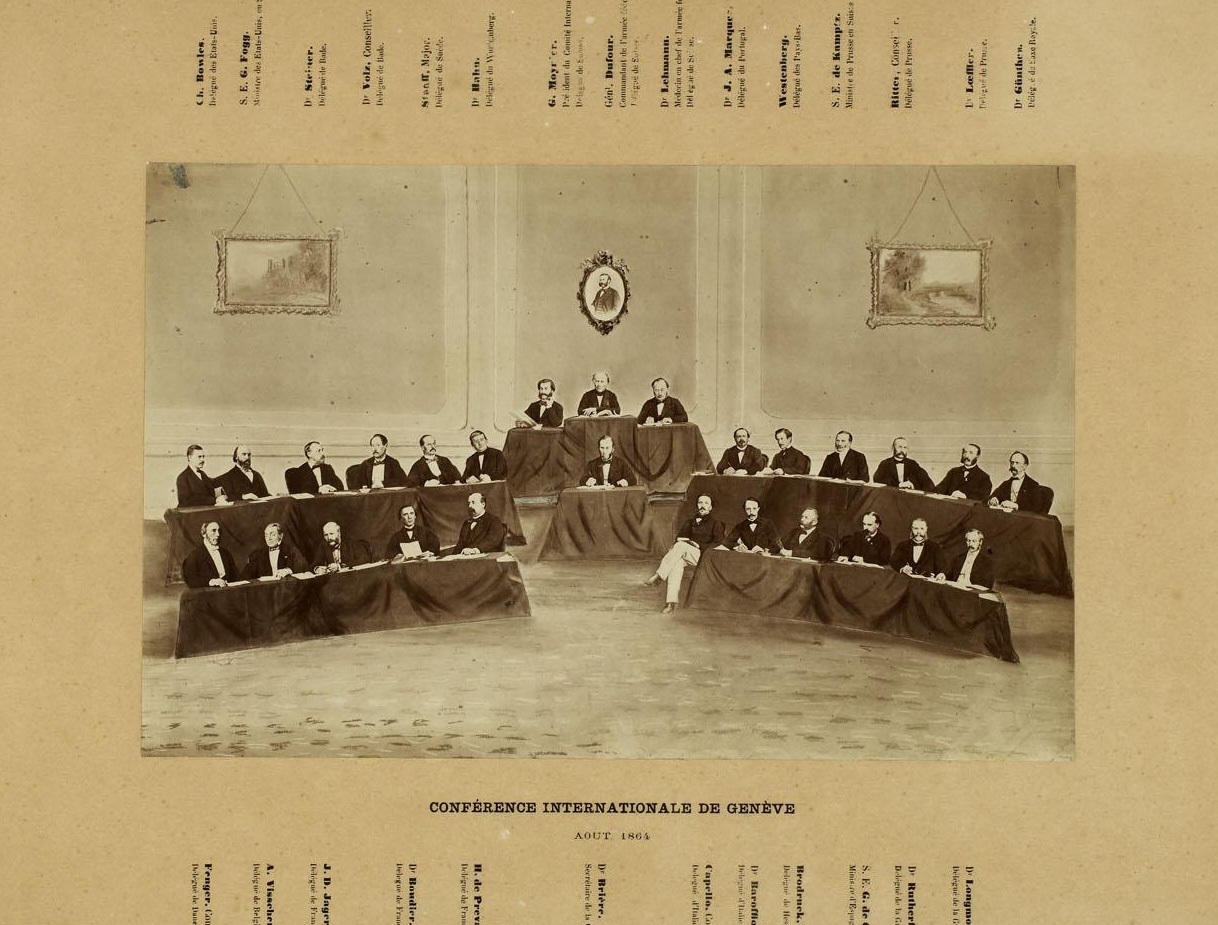
\includegraphics[keepaspectratio, height=\paperheight]{../img/geneva_convention.jpg}};
  \end{tikzpicture}
\end{frame}
% ----------------------------------------------------
% IMAGE NEEDED: geneva_convention.jpg -- fotografía histórica de la primera firma de la Convención de Ginebra (1864) o de la Cruz Roja en acción durante un conflicto; alternativamente, foto de los delegados en la conferencia de Ginebra de 1949
\note{Las Convenciones de Ginebra son el ejemplo más exitoso del derecho internacional humanitario. Surgieron de la iniciativa de Henry Dunant, un banquero suizo que presenció la batalla de Solferino en 1859 y quedó horrorizado por el sufrimiento de los heridos. Fundó la Cruz Roja y promovió el primer convenio de 1864. Hoy todos los 193 miembros de la ONU las han ratificado. Incluso en guerras brutales como la Segunda Guerra Mundial, los convenios influyeron en el trato a los prisioneros -- aunque con muchísimas violaciones. La clave: la reciprocidad. Los ejércitos tratan bien a los prisioneros enemigos esperando que el enemigo haga lo mismo con los suyos.}

% ----------------------------------------------------
\begin{frame}
\frametitle{Convenciones de Ginebra}
\centering

\begin{itemize}
  \item Primera Convención de Ginebra firmada en 1964
  \begin{itemize}
      \item Revisadas en 1906, 1929 y 1949
      \item Regulan derechos y protecciones de no combatientes, prisoneros de guerra, etc
  \end{itemize}
  \item Papel de Henry Dunant: empresario suizo que estuvo presente en la Batalla de Solferino (1859) y quedó horrorizado
  \begin{itemize}
      \item Fundó la Cruz Roja (1863) y promovió la primera convención
  \end{itemize}
  \item Hoy en día, firmadas por \textbf{todos los estados}
  \begin{itemize}
      \item Reciprocidad, reputación internacional, presión, moral...
  \end{itemize}
\end{itemize}

\end{frame}
% ----------------------------------------------------
\note{}

% ====================================================
\section{Normas internacionales}
% ====================================================

% ----------------------------------------------------
\begin{transitionframe}
Normas internacionales
\end{transitionframe}
% ----------------------------------------------------
\note{}

% ----------------------------------------------------
\begin{frame}
\frametitle{Normas: ¿qué son y cómo funcionan?}
\centering

\begin{itemize}
  \item \textbf{Normas:} estándares de comportamiento que una comunidad considera apropiados
  \item<2-> No son leyes --- pero condicionan las acciones de los Estados
  \begin{itemize}
    \item La violación exige \textit{justificación}
    \item La censura de otros revela la norma
  \end{itemize}
  \item<3-> Tres tipos:
  \begin{itemize}
    \item \textbf{Constitutivas:} definen quién es un actor legítimo
    \item \textbf{Procedimentales:} cómo tomar decisiones colectivas
    \item \textbf{Reguladoras:} cómo comportarse en las interacciones
  \end{itemize}
\end{itemize}

\end{frame}
% ----------------------------------------------------
\note{Las normas son más difusas que el derecho pero igual de importantes. No requieren codificación formal. Ejemplos clásicos:
\begin{itemize}
  \item \textbf{Tabú nuclear:} ningún Estado ha usado armas nucleares desde 1945, aunque al menos nueve las poseen. No es solo disuasión: los líderes evitan incluso contemplar su uso por miedo a ser considerados inmorales
  \item \textbf{Integridad territorial:} norma contra cambiar fronteras por la fuerza (desde 1945). Cuando Saddam Hussein invadió Kuwait en 1990, la comunidad internacional reaccionó. Cuando Rusia anexó Crimea en 2014, también -- aunque la respuesta fue más débil
  \item \textbf{Monitoreo electoral:} prácticamente desconocido antes de 1978, hoy todos los países democratizantes invitan observadores a sus primeras elecciones
\end{itemize}
Las normas se revelan mejor cuando se violan: el actor que las viola siente la necesidad de justificarse.}


% ----------------------------------------------------
\begin{frame}
\frametitle{Normas: ¿qué son y cómo funcionan?}
\centering

\begin{itemize}
  \item Muchas leyes empiezan como normas, que vienen de ideas sobre lo que está bien y mal
  \item Por lo general, la pregunta es cómo una idea que al principio puede parecer muy radical o marginal termina siendo adoptada por todos
\end{itemize}

\end{frame}
% ----------------------------------------------------
\note{}

% ----------------------------------------------------
\imageframe{../img/suffragettes}
\note{}
% ----------------------------------------------------

% ----------------------------------------------------
\imageframe{../img/abolitionism}
\note{}
% ----------------------------------------------------

% ----------------------------------------------------
\imageframe{../img/chemicalwwi}
\note{}
% ----------------------------------------------------

% ----------------------------------------------------
\imageframe{../img/chemicalwc}
\note{}
% ----------------------------------------------------

% ----------------------------------------------------
\imageframe{../img/landmines}
\note{}
% ----------------------------------------------------

% ----------------------------------------------------
\imageframe{../img/climate}
\note{}
% ----------------------------------------------------


% ----------------------------------------------------
\begin{frame}
\frametitle{El ciclo de vida de las normas}
\centering
\vspace{0.5em}

\resizebox{\textwidth}{!}{%
\begin{tikzpicture}[>=stealth, thick]
  % Stage boxes
  \node[draw, fill=accent!20, rounded corners, minimum width=2.5cm, minimum height=1.2cm, align=center] (s1) at (0,0) {\textbf{1. Emprendedores}\\\small de normas};
  \onslide<2->{\node[draw, fill=accent!40, rounded corners, minimum width=2.5cm, minimum height=1.2cm, align=center] (s2) at (4.5,0) {\textbf{2. Cascada}\\\small masa crítica};}
  \onslide<3->{\node[draw, fill=accent!70, rounded corners, minimum width=2.5cm, minimum height=1.2cm, align=center, text=white] (s3) at (9,0) {\textbf{3. Internalización}\\\small taken-for-granted};}

  % Arrows
  \onslide<2->{\draw[->] (s1) -- (s2);}
  \onslide<3->{\draw[->] (s2) -- (s3);}

  % Labels below (explicit coordinates)
  \node[align=center, font=\scriptsize] at (0, -1.1) {TANs, ONG,\\líderes morales};
  \onslide<2->{\node[align=center, font=\scriptsize] at (4.5, -1.1) {Punto de inflexión\\coerción / socialización};}
  \onslide<3->{\node[align=center, font=\scriptsize] at (9, -1.1) {La norma se vuelve\\``obvia''};}
\end{tikzpicture}}

\vspace{20pt}
{\small Finnemore \& Sikkink (1998)}

\end{frame}
% ----------------------------------------------------
\note{El modelo del ciclo de vida de las normas de Finnemore y Sikkink es una de las contribuciones más influyentes de las RRII constructivistas. Tres etapas:
\begin{enumerate}
  \item \textbf{Emprendedores de normas:} individuos y grupos que enmarcan un principio como moralmente correcto y buscan convencer a otros. El enmarcamiento es clave: conectar la nueva norma con valores ya aceptados. Ejemplo: los activistas contra las minas antipersona enmarcaron la cuestión como violencia contra civiles inocentes (niños que pierden piernas al pisar una mina años después del conflicto)
  \item \textbf{Cascada:} una vez que suficientes actores influyentes adoptan la norma, otros la siguen por conformidad (los Estados ``civilizados'' hacen X). El punto de inflexión es difícil de identificar de antemano
  \item \textbf{Internalización:} la norma se vuelve tan obvia que los actores ni siquiera contemplan violarla. El tabú contra el canibalismo es el ejemplo extremo; el tabú nuclear está cerca de este punto
\end{enumerate}
No todas las normas completan el ciclo. La prohibición del trabajo infantil, por ejemplo, sigue estancada entre las etapas 1 y 2.}

% ----------------------------------------------------
\begin{frame}
\frametitle{Redes transnacionales de activismo (TANs)}
\centering

\begin{columns}[T]
  \begin{column}{0.50\textwidth}
    \centering
    \textbf{\textcolor{accent}{¿Qué son?}}
    \begin{itemize}
      \item Redes de activistas y ONG en varios países
      \item Objetivos: derechos humanos, medio ambiente, justicia económica...
      \item Actores: ONG, fundaciones, medios, sindicatos, iglesias
    \end{itemize}
  \end{column}
  \begin{column}{0.46\textwidth}
    \centering
    \textbf{\textcolor{accent2}{¿Qué hacen?}}
    \begin{itemize}
      \item \textbf{Emprendedores de normas:} enmarcar y difundir
      \item \textbf{Avalistas:} informar a legisladores antes del acuerdo
      \item \textbf{Monitores:} vigilar el cumplimiento
      \item \textit{Naming \& shaming}
    \end{itemize}
  \end{column}
\end{columns}

\end{frame}
% ----------------------------------------------------
\note{Las TANs son el motor de la difusión de normas internacionales. Keck y Sikkink (1998) las estudian en su obra clásica ``Activists beyond Borders.'' Ejemplos:
\begin{itemize}
  \item \textbf{Campaña Internacional para Prohibir las Minas Antipersona (ICBL):} red de cientos de ONG en ~100 países. Negoció y logró la adopción del Tratado de Ottawa (1997). En 1997, la ICBL y su coordinadora Jody Williams recibieron el Premio Nobel de la Paz. Hoy 164 países lo han ratificado, aunque China, Rusia y EE.UU. se han quedado fuera
  \item \textbf{Greenpeace y Al Gore:} sobre el cambio climático. Las TANs han elevado la conciencia pública y presionado para el Acuerdo de París (2016)
  \item \textbf{Amnistía Internacional:} monitorea y denuncia violaciones de DDHH en todo el mundo
\end{itemize}
Las TANs son más eficaces como avalistas y monitores que como ejecutoras directas. Reducen la asimetría de información entre los Estados.}

% ----------------------------------------------------
\begin{frame}
\frametitle{El modelo ``bumerán''}
\centering
\vspace{0.8em}

\begin{tikzpicture}[>=stealth, thick, node distance=1.8cm]
  \node[draw, fill=accent2!20, rounded corners, align=center, minimum width=2.2cm, minimum height=0.9cm] (ngo1) at (0,0) {\small ONG\\\small (país A)};
  \node[draw, fill=accent!20, rounded corners, align=center, minimum width=2.2cm, minimum height=0.9cm] (gov1) at (0,-2.5) {\small Gobierno\\\small (país A)};
  \node[draw, fill=accent!20, rounded corners, align=center, minimum width=2.2cm, minimum height=0.9cm] (ngo2) at (6,0) {\small TANs\\\small internacionales};
  \only<2->{\node[draw, fill=accent2!20, rounded corners, align=center, minimum width=2.2cm, minimum height=0.9cm] (gov2) at (6,-2.5) {\small Gobierno\\\small (país B / OI)};}

  \draw[->, dashed, accent2, thick] (ngo1) -- node[right, xshift=2pt]{\scriptsize bloqueada} (gov1);
  \draw[->, accent, thick] (ngo1) -- node[above]{\scriptsize apela} (ngo2);
  \only<2->{\draw[->, accent, thick] (ngo2) -- (gov2);}
  \only<2->{\draw[->, accent2, thick] (gov2) -- node[above]{\scriptsize presión} (gov1);}
\end{tikzpicture}

\vspace{15pt}
\small Keck \& Sikkink (1998)

\end{frame}
% ----------------------------------------------------
\note{El modelo del bumerán explica cómo las ONG de países no democráticos pueden lograr cambios aunque su propio gobierno las bloquee. El proceso:
\begin{enumerate}
  \item Las ONG locales (país A) intentan presionar a su gobierno pero son reprimidas o ignoradas
  \item Activan sus vínculos transnacionales: contactan a ONG y TANs en países democráticos (país B)
  \item Esas TANs presionan a los gobiernos del país B y a organizaciones internacionales
  \item El gobierno del país B ejerce presión diplomática (sanciones, condicionalidad) sobre el gobierno del país A
\end{enumerate}
El caso más claro es el movimiento antiapartheid en Sudáfrica. Los grupos negros surafricanos, excluidos del poder, apelaron a sus aliados internacionales. Esas redes movilizaron a la opinión pública y a los gobiernos de los países occidentales, que impusieron sanciones. El resultado final: el fin del apartheid en 1990. Las redes sociales han acelerado el efecto bumerán al hacer posible transmitir instantáneamente vídeos de represión estatal a audiencias globales.}

% ----------------------------------------------------
\begin{frame}
\centering
\vspace{2em}

{\large ¿Ejemplo de una norma que esté hoy en la primera fase?}

\end{frame}
% ----------------------------------------------------
\note{Pausa de reflexión. Ejemplos posibles: la prohibición de las armas autónomas letales (robots asesinos), actualmente en fase de emprendedores (Campaña STOPKILLERROBOTS); las normas de responsabilidad empresarial en DDHH (Principios Rectores de la ONU, todavía soft law); las normas de ciberguerra. Conectar con el caso de las minas antipersona, que completó el ciclo completo con el Tratado de Ottawa (1997).}

% ====================================================
\section{Derechos humanos}
% ====================================================

% ----------------------------------------------------
\begin{transitionframe}
Derechos humanos
\end{transitionframe}
% ----------------------------------------------------
\note{}


% ----------------------------------------------------
\begin{frame}[plain]
  \begin{tikzpicture}[remember picture, overlay]
    \node[at = (current page.center), yshift = 0cm] (cover) {%
      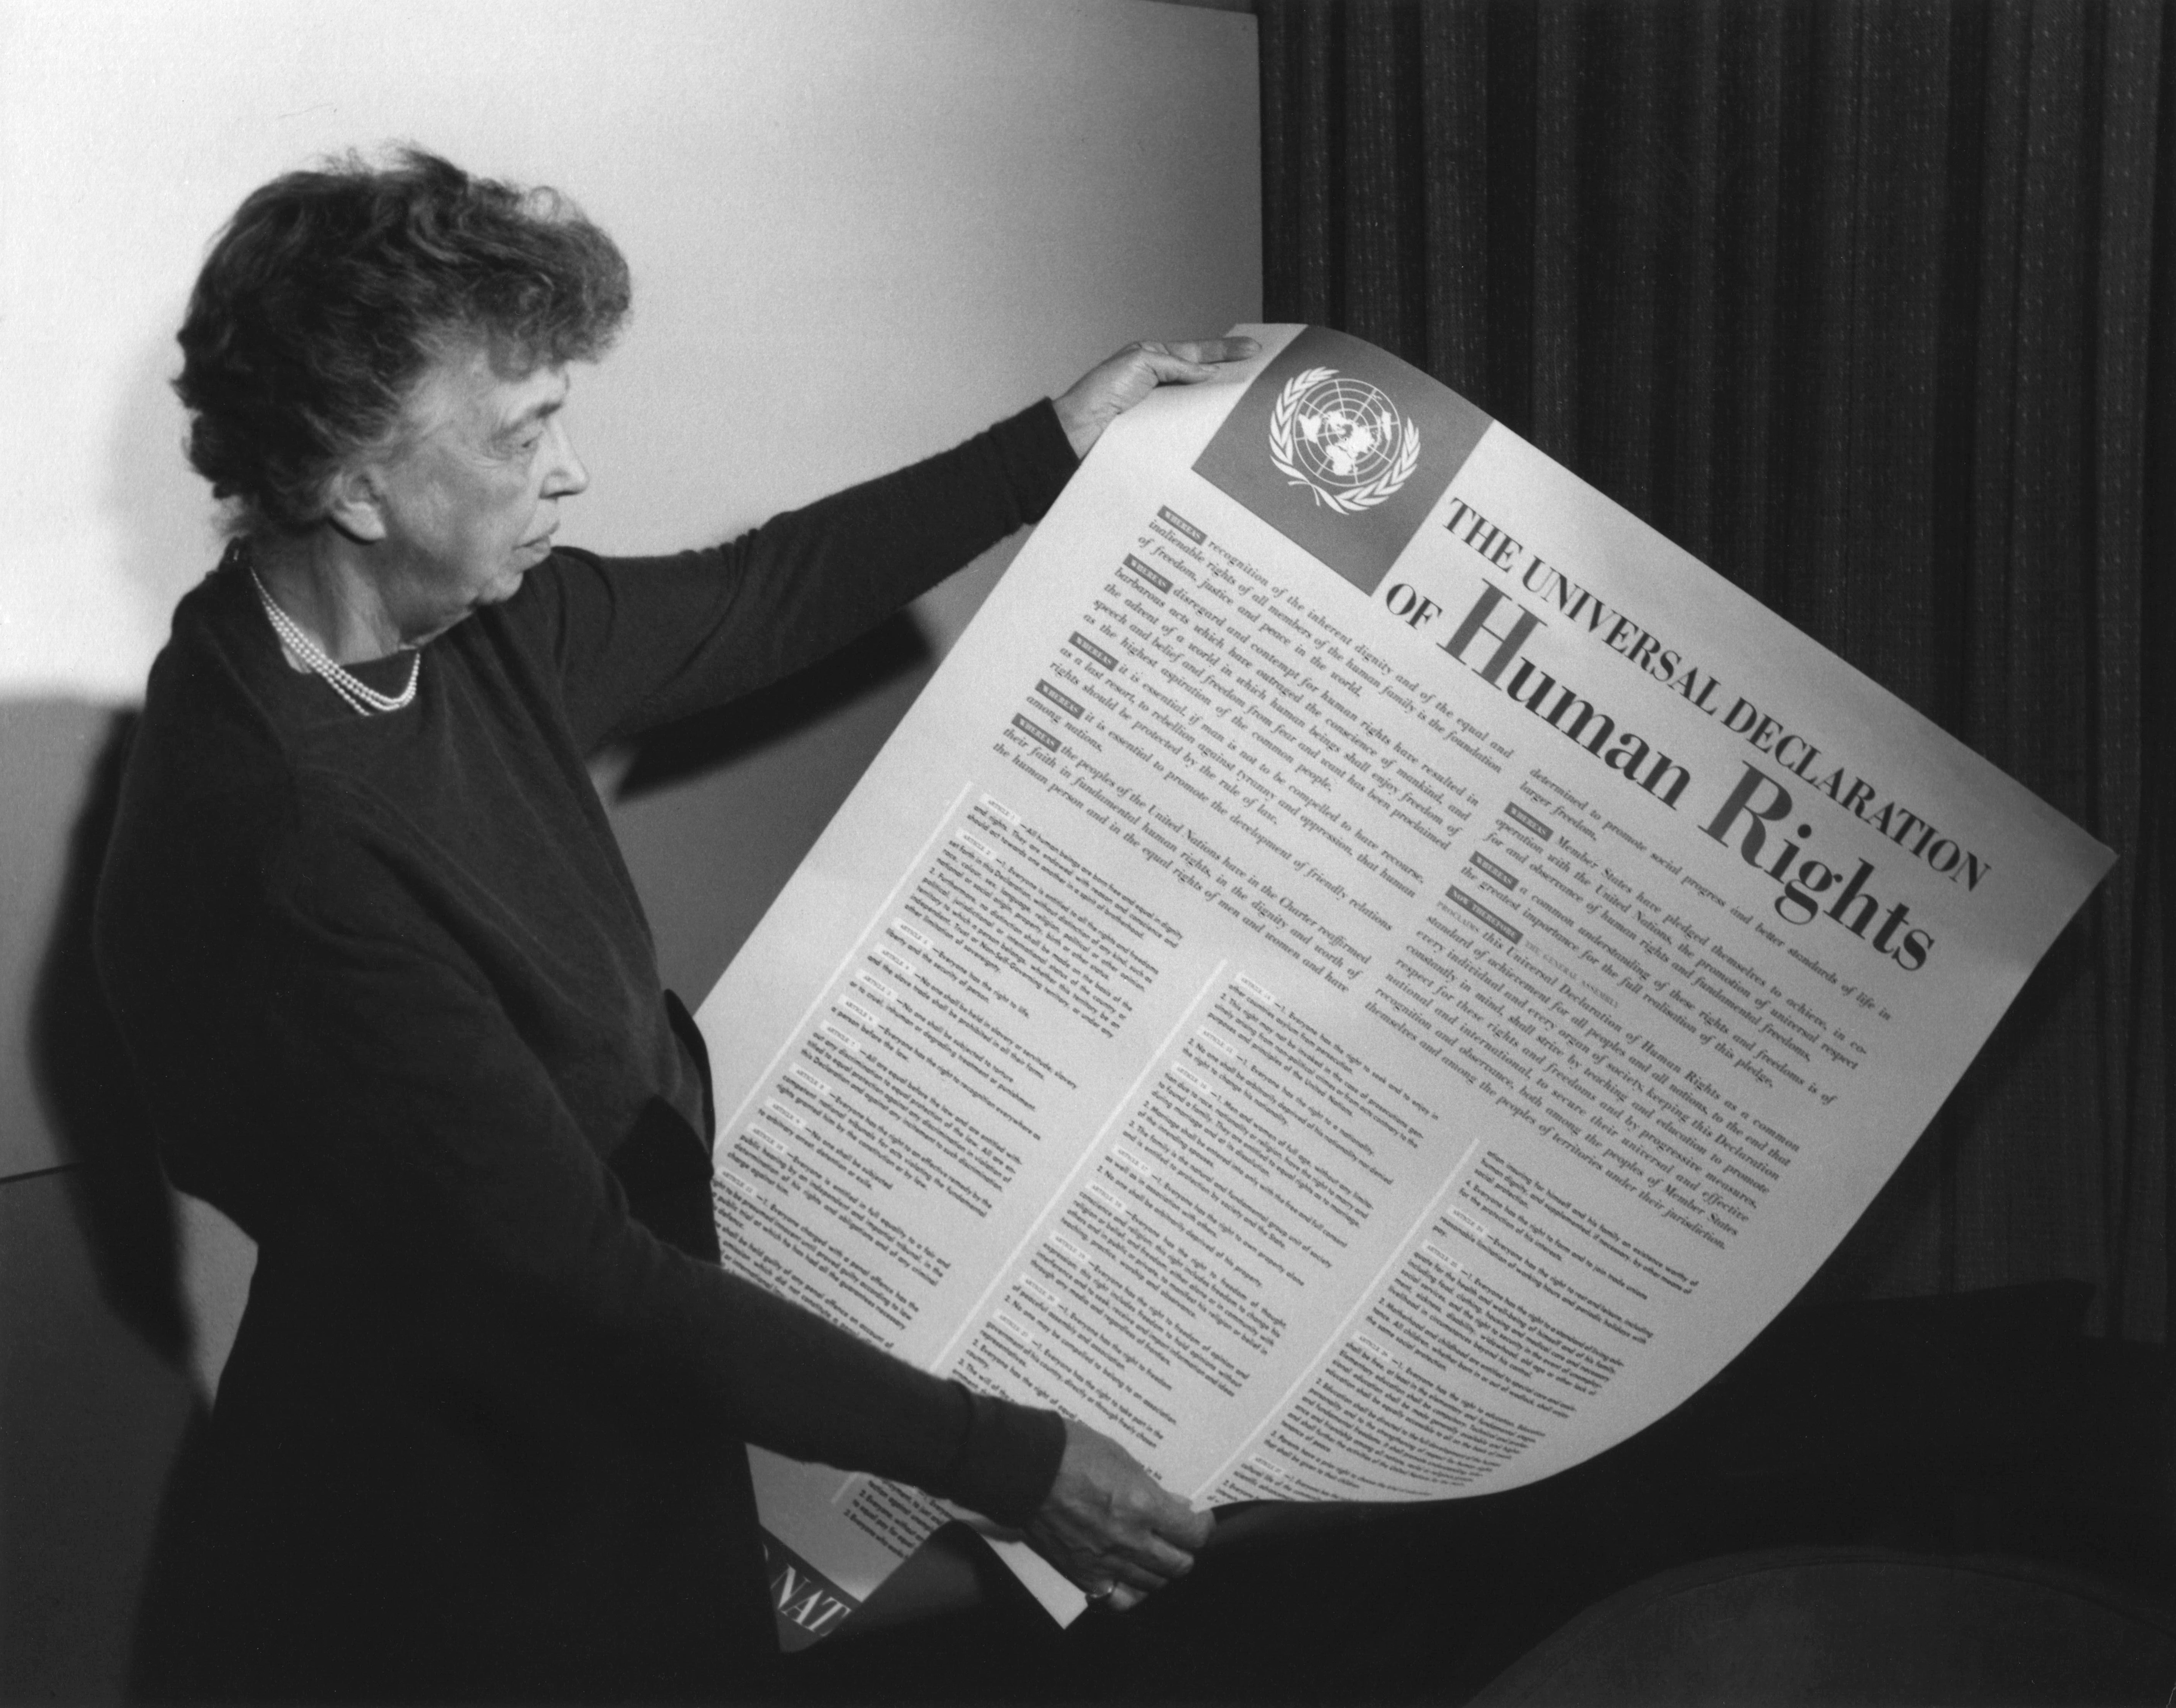
\includegraphics[keepaspectratio, height=\paperheight]{../img/udhr_signing.jpg}};
  \end{tikzpicture}
\end{frame}
% ----------------------------------------------------
% IMAGE NEEDED: udhr_signing.jpg -- fotografía de la proclamación de la Declaración Universal de Derechos Humanos en la ONU, diciembre de 1948; o retrato de Eleanor Roosevelt sosteniendo el documento de la DUDH
\note{La Declaración Universal de Derechos Humanos (DUDH), adoptada por la Asamblea General de la ONU el 10 de diciembre de 1948. Fue el producto directo del horror de la Segunda Guerra Mundial y el Holocausto. Eleanor Roosevelt presidió la comisión redactora. La DUDH no es un tratado vinculante (derecho blando), pero se ha convertido en el estándar de referencia del derecho internacional de los DDHH. 30 artículos que cubren un espectro amplísimo de derechos.}

% ----------------------------------------------------
\begin{frame}
\frametitle{¿Qué son los derechos humanos?}
\centering

\begin{itemize}
  \item Derechos que todo individuo posee \textbf{por el hecho de ser humano}
  \item Universales: independientes de la nacionalidad, grupo o estatus
  \item<2-> Tres ``generaciones'' de derechos:
  \begin{itemize}
    \item \textbf{1ª gen.:} civiles y políticos (Locke, Ilustración) --- libertad de expresión, proceso justo, no tortura
    \item \textbf{2ª gen.:} económicos, sociales, culturales (s.~XIX) --- trabajo, educación, salud
    \item \textbf{3ª gen.:} solidaridad y desarrollo (descolonización) --- autodeterminación, medio ambiente
  \end{itemize}
\end{itemize}

\end{frame}
% ----------------------------------------------------
\note{La genealogía filosófica de los DDHH arranca en la Ilustración: Locke formuló la idea de derechos naturales (vida, libertad, propiedad). Esta idea informó las revoluciones americana y francesa. La DUDH de 1948 organiza los derechos en torno a cuatro pilares (según René Cassin, uno de sus redactores): dignidad, libertad, igualdad y fraternidad. La división en tres generaciones refleja distintas tradiciones filosóficas y fue políticamente importante durante la Guerra Fría:
\begin{itemize}
  \item Los EE.UU. y los países occidentales enfatizaban los derechos civiles y políticos (1ª generación)
  \item La URSS y los países del bloque comunista enfatizaban los derechos económicos y sociales (2ª generación)
  \item Los países recién descolonizados añadieron los derechos colectivos (3ª generación)
\end{itemize}
Esta división llevó a la negociación de dos pactos separados en 1966, en vigor desde 1976: el PIDCP y el PIDESC.}

% ----------------------------------------------------
\begin{frame}
\frametitle{El régimen internacional de DDHH}
\centering

\footnotesize
\begin{tabular}{>{\bfseries}l p{5.5cm} l}
Año & Instrumento & Tipo \\
\hline
1948 & Declaración Universal de DDHH (DUDH) & Blando \\
1948 & Convención sobre el Genocidio & Duro \\
\only<2->{1966/76 & Pacto Internacional de Derechos Civiles y Políticos (PIDCP) & Duro \\}
\onslide<2->{1966/76 & Pacto Internacional de Derechos Económicos, Sociales y Culturales (PIDESC) & Duro \\}
\onslide<3->{1984 & Convención contra la Tortura (CAT) & Duro \\}
\onslide<4->{1998/2002 & Estatuto de Roma / Corte Penal Internacional (CPI) & Duro \\}
\end{tabular}

\vfill

\end{frame}
% ----------------------------------------------------
\note{Cronología del régimen internacional de DDHH. Observaciones clave:
\begin{itemize}
  \item La DUDH de 1948 es la base moral, pero es derecho blando. La Convención sobre el Genocidio (1948) fue el primer instrumento vinculante. Los EE.UU. firmaron la Convención en 1948 pero no la ratificaron hasta 1988
  \item El PIDCP y el PIDESC tardaron 18 años en negociarse y otros 10 en entrar en vigor. Reflejo de la división de la Guerra Fría
  \item La Convención contra la Tortura (1984) define la tortura con relativa precisión y prohíbe su uso de forma absoluta (es un derecho no derogable)
  \item La CPI/ICC (Estatuto de Roma, 1998; en vigor 2002) es la culminación: un tribunal permanente que puede juzgar a individuos por crímenes de guerra, crímenes contra la humanidad y genocidio. Notablemente, EE.UU., Rusia y China no son partes
\end{itemize}}

% ----------------------------------------------------
\begin{frame}
\frametitle{¿Son universales los DDHH? Depende quién responda}
\centering

\begin{columns}[T]
  \begin{column}{0.47\textwidth}
    \centering
    \textbf{\textcolor{accent}{A favor}}
    \begin{itemize}
      \item La dignidad humana trasciende culturas
      \item Los DDHH surgen del horror del Holocausto
      \item Aprobados por la casi totalidad de los Estados
    \end{itemize}
  \end{column}
  \begin{column}{0.47\textwidth}
    \centering
    \textbf{\textcolor{accent2}{Contra}}
    \begin{itemize}
      \item Origen occidental / liberal
      \item ``Valores asiáticos'': comunidad $>$ individuo
      \item Instrumento de interferencia política
    \end{itemize}
  \end{column}
\end{columns}

\vspace{15pt}
\onslide<2->{\small Los DDHH son un \textbf{campo de batalla político}, no solo un principio moral}
\onslide<3->{\small Críticas desde la izquierda y la derecha}

\end{frame}
% ----------------------------------------------------
\note{El debate sobre la universalidad de los DDHH es genuino y políticamente importante. Los argumentos en contra de la universalidad no son solo retórica de regímenes autoritarios:
\begin{itemize}
  \item Los filósofos comunitaristas (Confucio, y modernamente académicos como Michael Sandel) argumentan que los derechos del individuo no pueden entenderse fuera de su comunidad
  \item Los líderes de Singapur, Malasia e Indonesia argumentaron en los años 90 que los ``valores asiáticos'' (disciplina social, respeto a la autoridad, cohesión comunitaria) son incompatibles con algunos derechos civiles occidentales
  \item En la práctica, sin embargo, muchos de los líderes que invocan estos argumentos los usan para justificar la represión política, no para defender tradiciones culturales genuinas
\end{itemize}
La tensión real no es tanto entre culturas como entre soberanía e intervención: los Estados más reticentes a los DDHH internacionales son los que tienen más que perder si se aceptan mecanismos de rendición de cuentas externos.}


% ----------------------------------------------------
\begin{frame}[plain]
  \begin{tikzpicture}[remember picture, overlay]
    \node[at = (current page.center), xshift = -3cm] (cover) {%
      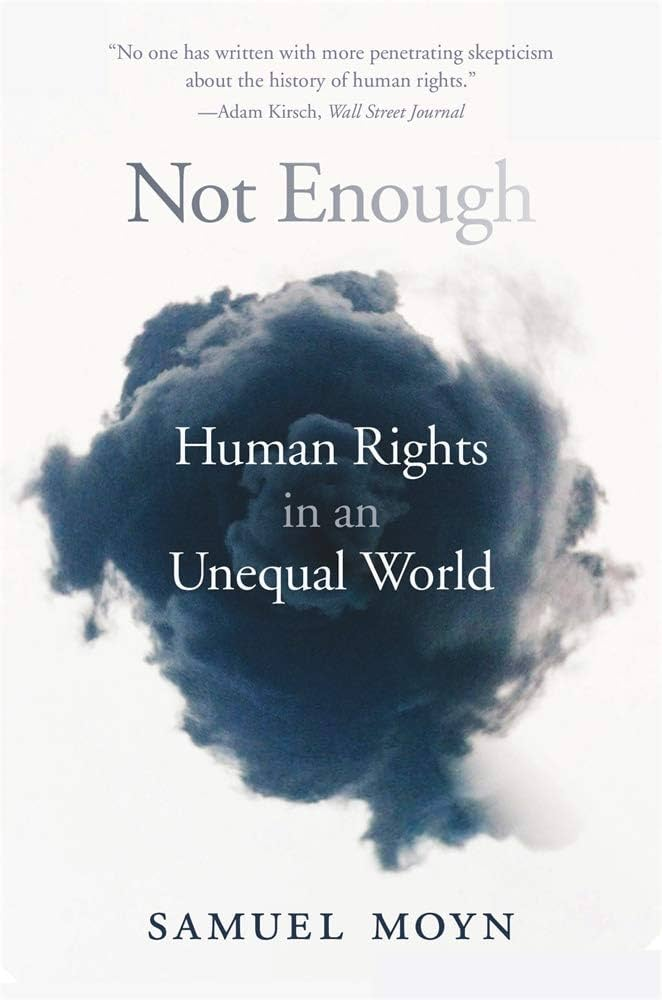
\includegraphics[keepaspectratio, height=\paperheight]{../img/moyn_not_enough}};
    \only<2->{\node[at = (current page.center), xshift = 3cm] (cover) {%
      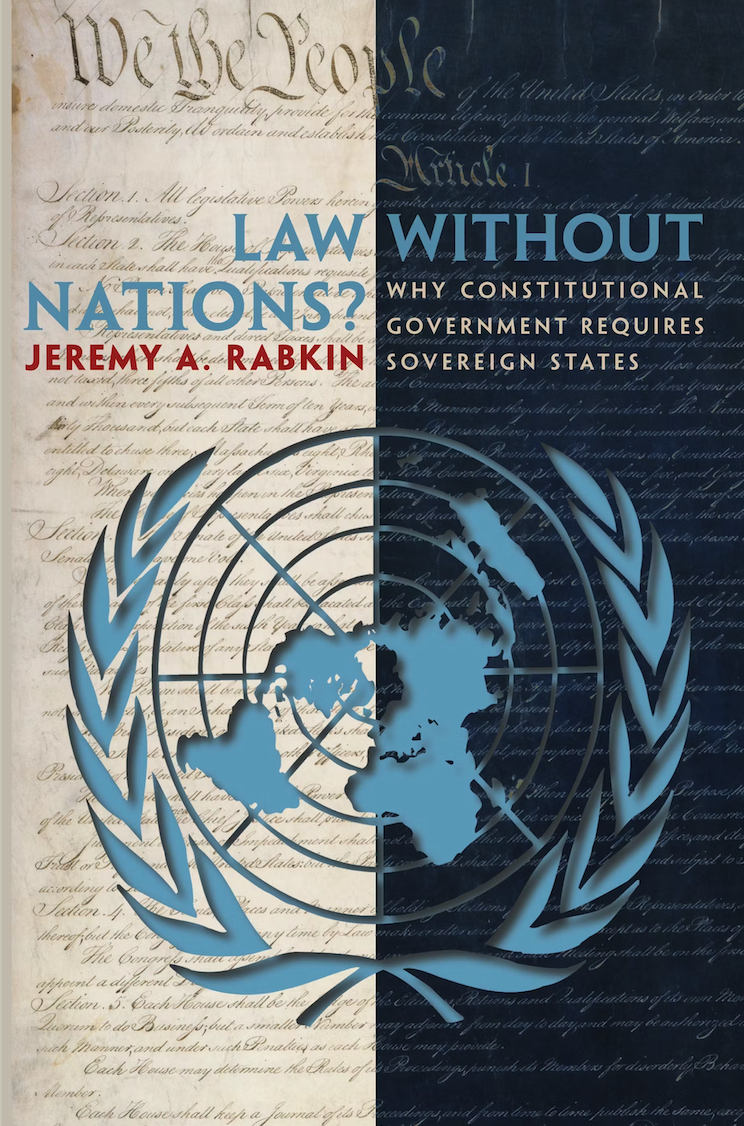
\includegraphics[keepaspectratio, height=\paperheight]{../img/rabkin_law_without_nations}};}
    \only<3->{\node[at = (current page.center), xshift = 3cm] (cover) {%
      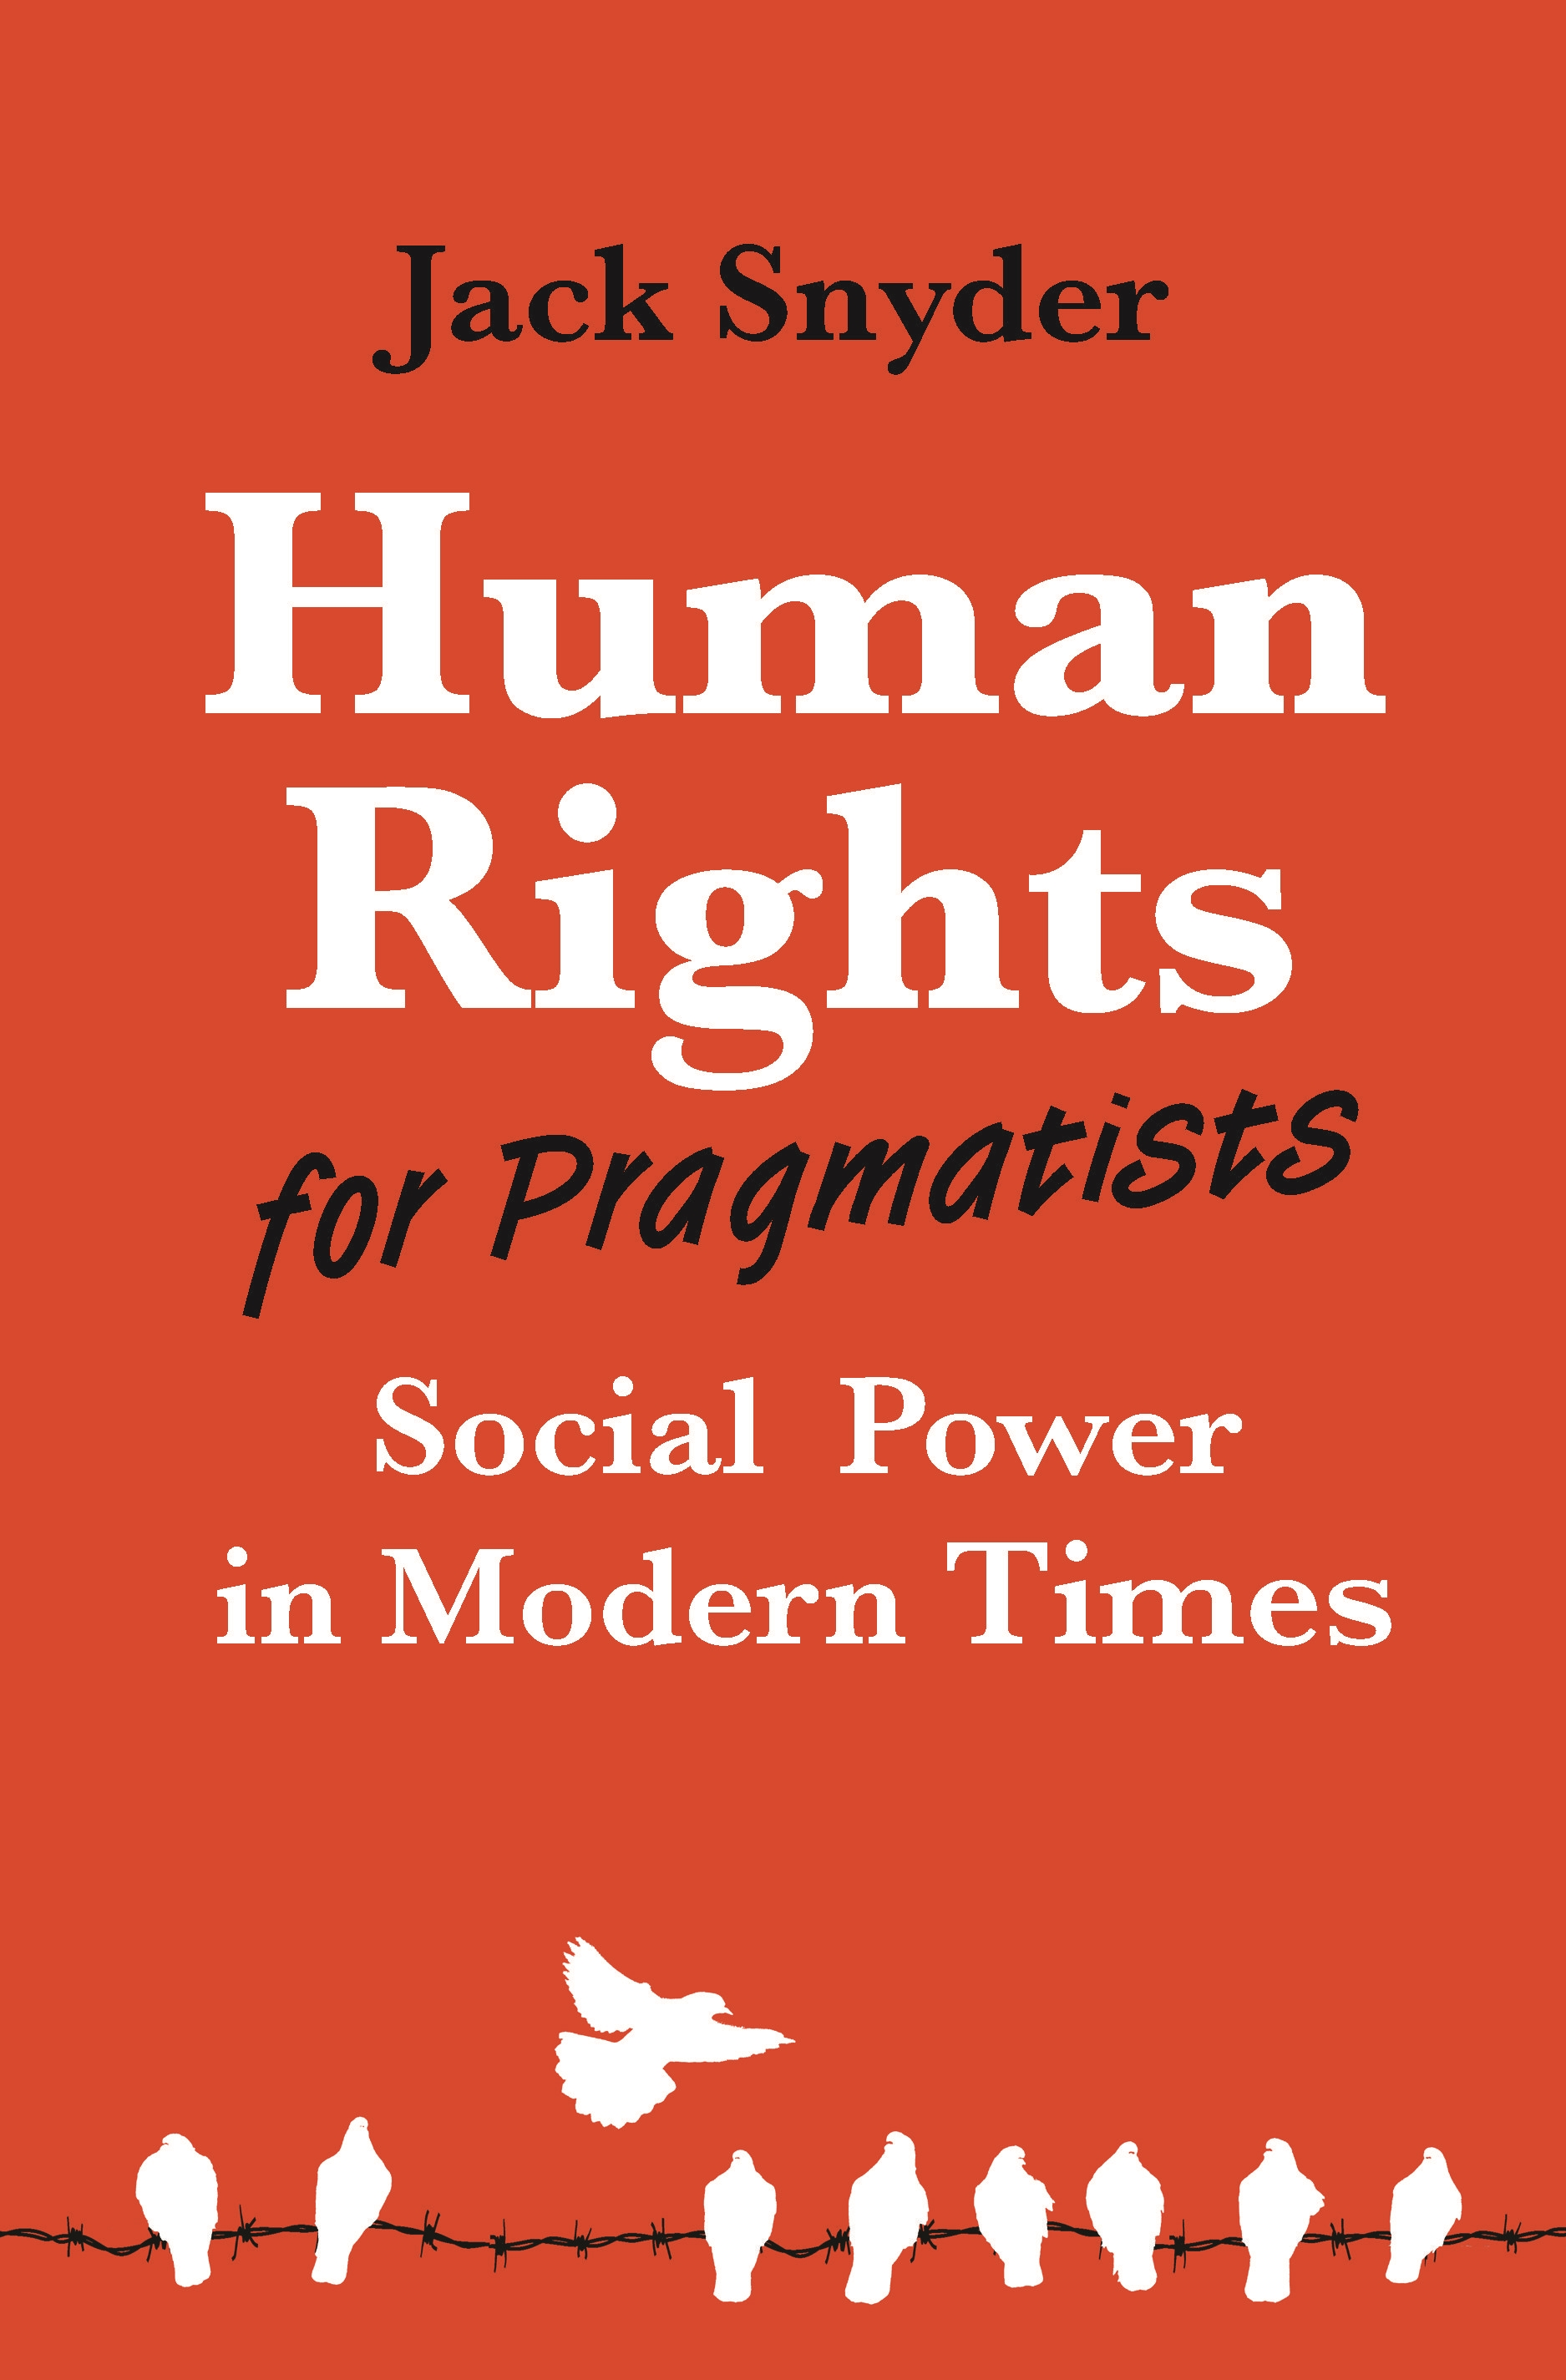
\includegraphics[keepaspectratio, height=\paperheight]{../img/snyder2022}};}
  \end{tikzpicture}
\end{frame}
% ----------------------------------------------------
\note{}

% % ----------------------------------------------------
% \begin{frame}
% \frametitle{¿Por qué violan derechos los Estados?}
% \centering

% \begin{itemize}
%   \item \textbf{Falta de capacidad:} no pueden garantizar los derechos aunque quieran
%   \item<2-> \textbf{Seguridad nacional:} la represión como respuesta a amenazas (reales o percibidas)
%   \begin{itemize}
%     \item EE.UU.: internamiento de japoneses-americanos (1942), Abu Ghraib (2004)
%   \end{itemize}
%   \item<3-> \textbf{Supervivencia del régimen:} reprimir a la oposición para mantenerse en el poder
%   \begin{itemize}
%     \item Argentina: ``Guerra Sucia'' (1976--83) -- ~10.000 desaparecidos
%     \item Ruanda: genocidio tutsi (1994) -- ~800.000 muertos en 100 días
%   \end{itemize}
% \end{itemize}

% \end{frame}
% % ----------------------------------------------------
% \note{Tres razones por las que los Estados violan los DDHH:
% \begin{enumerate}
%   \item \textbf{Capacidad:} muchos países pobres no pueden financiar escolarización universal (exigida por el PIDESC). O no controlan suficientemente a sus fuerzas de seguridad. Abu Ghraib: abuso por soldados actuando aparentemente de manera autónoma, no como política oficial (aunque esta distinción es discutida)
%   \item \textbf{Seguridad nacional:} en situaciones de guerra real o percibida, los Estados tienden a restringir derechos. Los internados japoneses-americanos durante la WWII. El debate sobre la tortura en la ``guerra contra el terror'' tras el 11-S. En todos los casos, el Estado argumenta que la seguridad es prioritaria
%   \item \textbf{Supervivencia del régimen:} el caso más puro. La dictadura militar argentina secuestró, torturó y asesinó a unos 10.000 opositores. Los ``vuelos de la muerte'' (arrojar prisioneros al océano desde aviones). El genocidio en Ruanda: los extremistas hutus utilizaron la radio para coordinar el asesinato sistemático de tutsis. Los regímenes autoritarios o semiautoritarios son significativamente más propensos a violar DDHH
% \end{enumerate}}

% ----------------------------------------------------
\begin{frame}
\frametitle{¿Por qué firman los acuerdos de DDHH?}
\centering

\begin{itemize}
  \item[] Está claro por qué los Estados violan derechos, ¿pero por qué se atan las manos y firman los acuerdos?
  \item<2-> \textbf{Compromiso sincero:} algunos gobiernos genuinamente creen en los derechos
  \item<3-> \textbf{Bloquear retrocesos}: los gobiernos democratizantes se ``atan'' para impedir regresiones futuras
  \begin{itemize}
    \item Las democracias nuevas firman más tratados que las consolidadas
  \end{itemize}
  \item<4-> \textbf{Señalización:} aparentar cumplimiento sin cambiar conducta
  \begin{itemize}
    \item ``Valor expresivo'' --- firma para ganar reputación internacional
  \end{itemize}
  \item<5-> \textbf{Condicionalidad:} firmar para recibir ayuda, acceso a la UE...
\end{itemize}

\end{frame}
% ----------------------------------------------------
\note{La paradoja del cumplimiento en DDHH: a veces los países que más violan derechos son los que más tratados firman. Vreeland (2008) muestra que las dictaduras multipartidistas tanto firman la CAT como utilizan la tortura más que la media. ¿Por qué? Porque la oposición doméstica presiona para firmar, pero el régimen sigue torturando porque necesita reprimir para sobrevivir. Tres explicaciones alternativas para la firma:
\begin{itemize}
  \item Moravcsik: los nuevos demócratas de Europa del Sur y del Este firmaron la TEDH para protegerse contra posibles golpes futuros. Es una forma de comprometerse creíblemente con la democracia
  \item Señalización pura: algunos Estados firman para parecer ``civilizados'' ante la comunidad internacional pero sin intención de cambiar conducta. Hathaway lo llama el ``valor expresivo'' de los tratados
  \item Condicionalidad: la UE exigió la ratificación de la Convención Europea de DDHH y otros tratados como condición de adhesión. Turquía ha tenido que mejorar su récord de DDHH (especialmente con los kurdos) como condición para las negociaciones de adhesión
\end{itemize}}

% ----------------------------------------------------
\begin{frame}
\frametitle{¿Funciona el derecho internacional de DDHH?}
\centering

\begin{itemize}
  \item El vaso está \textbf{medio lleno y medio vacío}
  \item<2-> Las violaciones masivas siguen ocurriendo
  \begin{itemize}
    \item La forma más mortífera de violencia hoy: \textit{gobiernos contra sus propios ciudadanos}
  \end{itemize}
  \item<3-> Pero hay evidencia de mejora condicionada:
  \begin{itemize}
    \item Los tratados funcionan \textit{si} hay tribunales domésticos fuertes
    \item Los tratados funcionan \textit{si} hay muchas ONG activas
    \item La amenaza de castigo sí parece hacer que algunos actores (estados y no estados) no cometan tantas violaciones
    \item A largo plazo: el ejemplo de Helsinki (1975) y la caída del comunismo, o la Convención de la Tortura (1983) y Pinochet
  \end{itemize}
\end{itemize}

\end{frame}
% ----------------------------------------------------
\note{El debate académico sobre la eficacia del derecho internacional de DDHH es uno de los más vivos en las RRII. Puntos clave:
\begin{itemize}
  \item Hathaway (2002): encontró que firmar tratados de DDHH se asocia con \textit{peores} prácticas, controlando por otras variables. Explicación: los países que más necesitan señalizar que son ``buenos'' (dictaduras) son los que firman más
  \item Simmons (2009): resultado más optimista: los tratados pueden movilizar actores domésticos (abogados, ONG, jueces) que presionan desde dentro. El efecto es mayor en democracias parciales que en democracias consolidadas o en dictaduras puras
  \item El caso del Acuerdo de Helsinki (1975): la URSS aceptó la mención de derechos humanos en el acta final a cambio de reconocimiento de las fronteras de posguerra. Esta concesión aparentemente menor terminó siendo un catalizador para los disidentes en Europa del Este. Tres años después, Solidaridad en Polonia; catorce después, la caída del Muro de Berlín
\end{itemize}
Conclusión: el efecto existe, pero es contingente, indirecto y a largo plazo.}

% % ----------------------------------------------------
% \begin{frame}
% \centering
% \vspace{2em}

% {\large Si los tratados de DDHH no siempre mejoran el comportamiento de los Estados,\\[0.5em]\textit{¿sirve de algo firmarlos?}}

% \end{frame}
% % ----------------------------------------------------
% \note{Pausa de reflexión. Invitar a los estudiantes a aplicar las tres razones por las que los Estados firman tratados: compromiso sincero, bloquear retrocesos (Moravcsik), señalización. La evidencia de Simmons: los tratados funcionan donde hay actores domésticos que presionan --- ONG, jueces, movimientos sociales. La respuesta no es sí/no sino contingente: depende del régimen, la sociedad civil y los mecanismos de implementación.}

% % ====================================================
% \section{R2P: la tensión entre soberanía y DDHH}
% % ====================================================

% % ----------------------------------------------------
% \begin{transitionframe}
% Responsabilidad de Proteger (R2P)
% \end{transitionframe}
% % ----------------------------------------------------
% \note{}

% ----------------------------------------------------
\begin{frame}
\frametitle{Soberanía y DDHH}
\centering

\begin{itemize}
  \item ¿Qué pasa cuando los DDHH o el derecho internacional entran en conflicto con la soberanía?
  \item Responsabilidad de Proteger (R2P)
  \item Muchos ejemplos de este debate:
  \begin{itemize}
      \item La actual guerra de Irán
      \item Gaza (2023--)
      \item Iraq (2003)
      \item Kosovo (1999)
      \item ...
  \end{itemize}
\end{itemize}

\end{frame}
% ----------------------------------------------------
\note{}

% ----------------------------------------------------
\begin{frame}[plain]
  \begin{tikzpicture}[remember picture, overlay]
    \node[at = (current page.center), yshift = 0cm] (cover) {%
      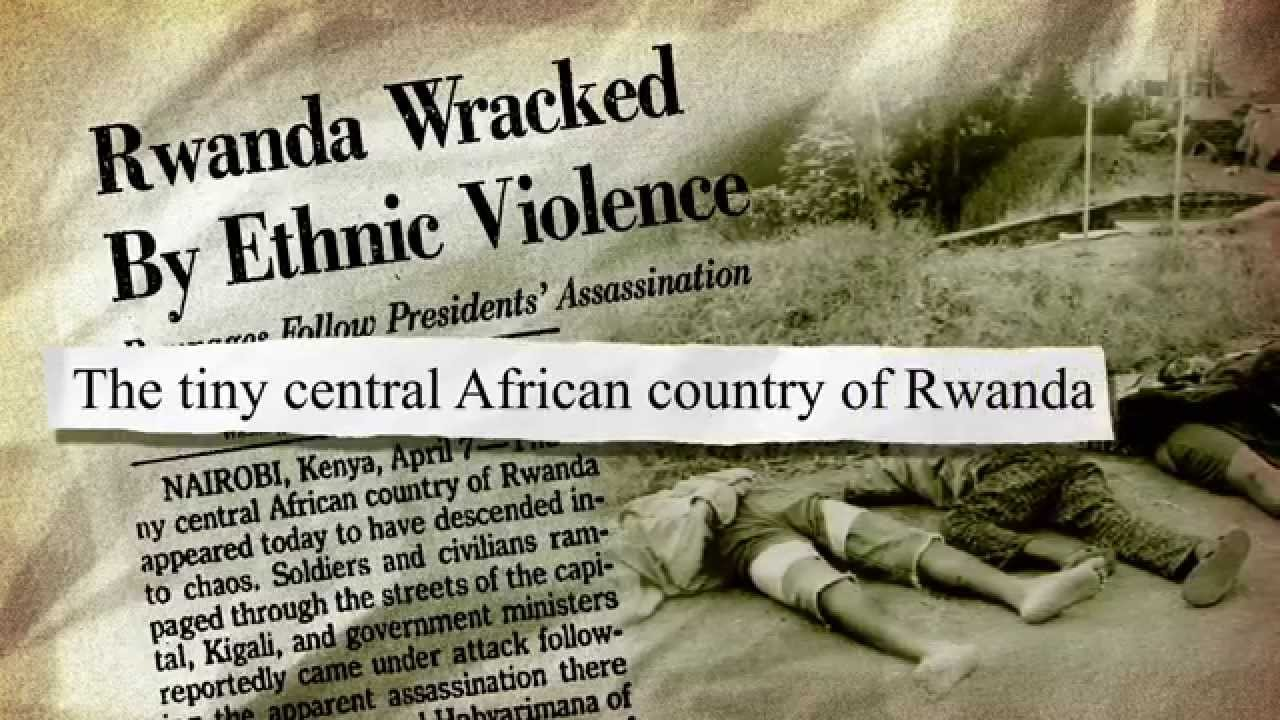
\includegraphics[keepaspectratio, width=\paperwidth]{../img/rwanda_genocide.jpg}};
  \end{tikzpicture}
\end{frame}
% ----------------------------------------------------
% IMAGE NEEDED: rwanda_genocide.jpg -- fotografía del genocidio de Ruanda de 1994 (víctimas, refugiados, o el cementerio de Kigali); o foto de Kofi Annan visitando Ruanda en los años posteriores
\note{El genocidio de Ruanda (1994): ~800.000 personas (principalmente tutsis) asesinadas en 100 días. La comunidad internacional observó y condenó pero no intervino. Una pequeña fuerza de la ONU ya desplegada en el país fue desbordada. El general canadiense Roméo Dallaire, comandante de esa fuerza, envió el infame fax a la ONU advirtiendo del genocidio inminente -- y la ONU le ordenó que no actuara. Este fracaso marcó a toda una generación de responsables de política exterior. El entonces Secretario General Kofi Annan lanzó en 1999 el reto: ¿cuándo tiene la comunidad internacional la responsabilidad de proteger a las poblaciones en peligro?}

% ----------------------------------------------------
\begin{frame}
\frametitle{La Responsabilidad de Proteger (R2P)}
\centering

\begin{itemize}
  \item Impulsada por el fracaso de Ruanda (1994) y Kosovo (1999)
  \item<2-> La Comisión Internacional sobre Intervención y Soberanía del Estado (2001): la soberanía conlleva \textbf{responsabilidad}
  \item<3-> Si un Estado no puede o no quiere proteger a su población:
  \begin{itemize}
    \item La responsabilidad \textit{recae} en la comunidad internacional
    \item Intervención militar como \textbf{último recurso}
    \item[] (Esto es \textbf{importante}: papel de la diplomacia y los ataques en Irán)
  \end{itemize}
  \item<4-> Aprobado por el Consejo de Seguridad de la ONU en 2006
\end{itemize}

\end{frame}
% ----------------------------------------------------
\note{La R2P fue desarrollada por la Comisión Internacional sobre Intervención y Soberanía del Estado (ICISS), patrocinada por Canadá en 2000. El informe ``La Responsabilidad de Proteger'' (2001) supuso un giro conceptual:
\begin{itemize}
  \item Antes: la soberanía como escudo absoluto -- los asuntos internos son intocables
  \item Después: la soberanía como responsabilidad -- si el Estado falla en proteger a su población, la comunidad internacional puede actuar
\end{itemize}
La R2P distingue tres responsabilidades: prevenir, reaccionar y reconstruir. La intervención militar es el último recurso, no el primero. El Consejo de Seguridad de la ONU avaló la R2P en la Cumbre Mundial de 2005 y en la Resolución 1674 (2006). Pero es una \textbf{norma}, no un tratado: ningún Estado ha aceptado formalmente que puede ser intervenido en su contra. La tensión con la soberanía sigue siendo enorme.}

% ----------------------------------------------------
\begin{frame}
\frametitle{R2P en la práctica: ¿funciona?}
\centering

\begin{columns}[T]
  \begin{column}{0.47\textwidth}
    \centering
    \textbf{\textcolor{accent}{Aplicada}}
    \begin{itemize}
      \item Libia (2011): OTAN interviene con mandato del CS-ONU
      \item Sudán del Sur, Mali: misiones de paz
    \end{itemize}
  \end{column}
  \begin{column}{0.47\textwidth}
    \centering
    \textbf{\textcolor{accent2}{Bloqueada}}
    \begin{itemize}
      \item Siria: veto ruso y chino en el CS-ONU
      \item Yemen, Myanmar: intervención no autorizada
      \item Gaza: debate abierto (2023--)
    \end{itemize}
  \end{column}
\end{columns}

\vspace{12pt}
\onslide<2->{\small El poder de veto sigue siendo el principal obstáculo}

\end{frame}
% ----------------------------------------------------
\note{La R2P ha tenido una aplicación muy desigual:
\begin{itemize}
  \item \textbf{Libia (2011):} el caso más claro. El CS-ONU autorizó la intervención de la OTAN para proteger a la población civil de Gadafi. Pero la operación fue más allá de la protección y acabó con el régimen. Rusia y China, que se habían abstenido, protestaron por este exceso y vetaron cualquier acción similar en Siria
  \item \textbf{Siria:} el caso de fracaso más evidente. El régimen de Assad usó armas químicas contra civiles. Pero los vetos rusos y chinos bloquearon cualquier acción del CS-ONU. EE.UU. lanzó ataques con misiles en 2017 y 2018, pero de forma unilateral y sin mandato de la ONU
  \item \textbf{Gaza (2023-24):} debate intenso sobre si la respuesta israelí supera el umbral para la aplicación de la R2P. La CIJ dictó medidas cautelares en el caso de genocidio presentado por Sudáfrica
\end{itemize}
La lección: la R2P como norma existe, pero su aplicación depende de la geometría de poder en el CS-ONU y de los intereses de las grandes potencias.}

% ----------------------------------------------------
\begin{frame}
\frametitle{El dilema: soberanía vs.~derechos humanos}
\centering
\vspace{0.8em}

\begin{tikzpicture}[>=stealth, thick]
  \node[draw, fill=accent!20, rounded corners, minimum width=3.5cm, minimum height=1.2cm, align=center] (sov) at (-3,0) {\textbf{Soberanía}\\\small no intervención};
  \node[draw, fill=accent2!20, rounded corners, minimum width=3.5cm, minimum height=1.2cm, align=center] (hr) at (3,0) {\textbf{DDHH}\\\small responsabilidad};
  \node[draw=asher, dashed, rounded corners, minimum width=2cm, minimum height=1cm, align=center] (r2p) at (0,-2) {\small R2P};

  \draw[<->, thick, color=asher] (sov) -- (hr);
  \draw[->, dashed, color=asher] (r2p) -- (0,-0.5);
\end{tikzpicture}

\vspace{6pt}
\begin{itemize}
  \item<2-> ¿Tiene la comunidad internacional derecho a intervenir en asuntos internos?
  \item<3-> ¿Quién decide cuándo se supera el umbral?
\end{itemize}

\end{frame}
% ----------------------------------------------------
\note{La tensión entre soberanía y DDHH es estructural en el sistema internacional. La soberanía implica que los asuntos internos son intocables; los DDHH implican que hay estándares universales que ningún Estado puede violar impunemente. La R2P intenta bridgear esta tensión, pero no la resuelve:
\begin{itemize}
  \item Si la soberanía es absoluta: Ruanda, el Holocausto, Camboya son ``asuntos internos''
  \item Si los DDHH son absolutos: ¿quién decide cuándo intervenir? ¿El CS-ONU con su poder de veto? ¿Las grandes potencias? El riesgo de que la intervención humanitaria sea un disfraz del imperialismo
  \item Los alemanes tuvieron este dilema en Kosovo: su compromiso con ``nunca más'' (genocidio) chocó con su compromiso con ``nunca más'' (guerra). Finalmente apoyaron la intervención de la OTAN
\end{itemize}
No hay respuesta fácil. El principio de R2P representa un progreso moral real, pero su aplicación es profundamente política.}

% ====================================================
\section{Instituciones internacionales de DDHH}
% ====================================================

% ----------------------------------------------------
\begin{transitionframe}
Justicia Transitional y mecanismos de rendición de cuentas
\end{transitionframe}
% ----------------------------------------------------
\note{}

% ----------------------------------------------------
\begin{frame}[plain]
  \begin{tikzpicture}[remember picture, overlay]
    \node[at = (current page.center), yshift = 0cm] (cover) {%
      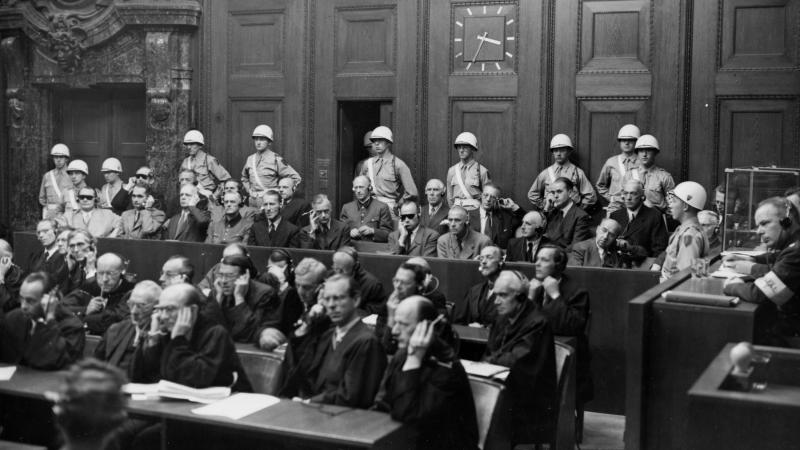
\includegraphics[keepaspectratio, height=\paperheight]{../img/nuremberg.jpeg}};
  \end{tikzpicture}
\end{frame}
% ----------------------------------------------------
\note{El Tribunal Militar Internacional de Núremberg (1945-46): primer tribunal internacional que juzgó a individuos por crímenes de guerra, crímenes contra la paz y crímenes contra la humanidad. 24 altos cargos nazis. 12 condenas a muerte. Principio clave: la obediencia a órdenes superiores no exime de responsabilidad. Fue controversial (``justicia de los vencedores''), pero sentó las bases del derecho penal internacional moderno.}

% ----------------------------------------------------
\begin{frame}
\frametitle{De Núremberg a la CPI: el arco histórico}
\centering
\vspace{0.8em}

\resizebox{\textwidth}{!}{%
\begin{tikzpicture}[>=stealth, thick]
  \draw[thick] (0,0) -- (11,0);

  \foreach \x/\lab in {0/1945, 3.5/1985, 6/1993, 8/1998, 11/2002} {
    \draw (\x, -0.15) -- (\x, 0.3);
    \node[above, font=\scriptsize\bfseries] at (\x, 0.28) {\lab};
  }

  \node[below, font=\scriptsize, align=center, text=accent2] at (0,-0.2)
    {Núremberg\\\textit{(intl.)}};
  \node[below, font=\scriptsize, align=center, text=accent] at (3.5,-0.2)
    {Argentina\\\textit{(doméstico)}};
  \node[below, font=\scriptsize, align=center, text=accent2] at (6,-0.2)
    {TPIY\\\textit{(intl.)}};
  \node[below, font=\scriptsize, align=center, text=asher] at (8,-0.2)
    {Pinochet\\\textit{(extranjero)}};
  \node[below, font=\scriptsize, align=center, text=accent] at (11,-0.2)
    {CPI/ICC\\\textit{(permanente)}};
\end{tikzpicture}}

\vspace{8pt}
{\scriptsize \textcolor{accent2}{$\blacksquare$} internacional \quad \textcolor{accent}{$\blacksquare$} doméstico/extranjero \quad \textcolor{asher}{$\blacksquare$} extranjero}

\vspace{15pt}
\begin{itemize}
    \item<2-> Otros pioneros por el medio: Grecia (1975), Portugal (1974, ej. PIDE)
    \item<3-> Cada hito expande la norma: más actores, más tipos de delitos, más jurisdicciones
\end{itemize}

\end{frame}
% ----------------------------------------------------
\note{El arco histórico de la justicia internacional:
\begin{itemize}
  \item \textbf{Núremberg (1945-46):} primer tribunal penal internacional; nuevos conceptos (crímenes contra la humanidad, crímenes contra la paz)
  \item \textbf{Argentina (1985):} primer juicio doméstico a los líderes de una dictadura por violaciones de DDHH (Juicio a las Juntas)
  \item \textbf{TPIY (1993):} Tribunal Penal Internacional para la ex Yugoslavia. Juzgó a Milošević, condenó a Radovan Karadžić
  \item \textbf{Pinochet (1998):} el juez español Baltasar Garzón emitió una orden de arresto internacional. Primer caso importante de jurisdicción extranjera sobre un jefe de Estado
  \item \textbf{CPI/ICC (2002):} primer tribunal permanente con jurisdicción universal
\end{itemize}}

% ----------------------------------------------------
\begin{frame}
\frametitle{La Cascada de Justicia}
\centering

\begin{itemize}
  \setlength{\itemsep}{8pt}
  \item Una nueva norma internacional:
  \item[] la \textbf{responsabilidad criminal individual}
  \begin{itemize}
    \item Los líderes son personalmente responsables de las violaciones de DDHH (no inmunidad, ni el Estado)
  \end{itemize}
  \item<2-> Tres tipos de tribunales que la aplican:
  \begin{itemize}
    \item \textbf{Domésticos:} el país juzga sus propias violaciones (Argentina, 1985)
    \item \textbf{Extranjeros:} otro país ejerce jurisdicción (Pinochet en Londres)
    \item \textbf{Internacionales:} tribunales ad hoc o la CPI
  \end{itemize}
  \item<3-> Los tres tipos de juicios han crecido exponencialmente desde los años 80
  \item<4-> Motor: redes de activistas, abogados y ONG --- la misma lógica que las TANs
\end{itemize}

\vspace{4pt}
\small\textcolor{asher}{Sikkink (2011)}

  \begin{tikzpicture}[remember picture, overlay]
    \only<5->{\node[at = (current page.center), yshift = 0cm] (cover) {%
      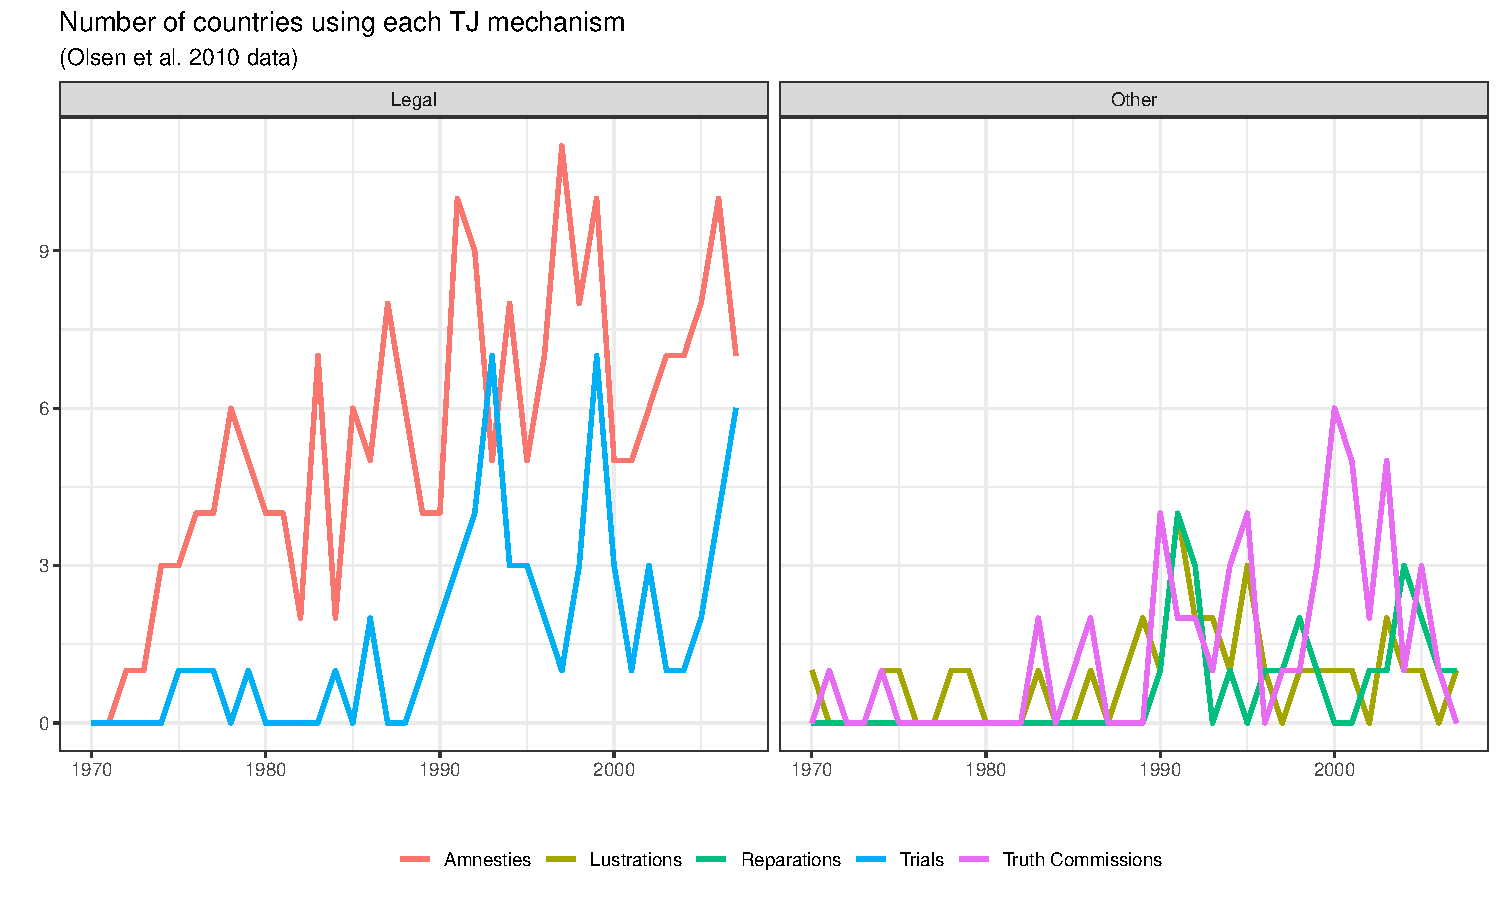
\includegraphics[keepaspectratio, height=0.9\paperheight]{../img/countries_by_year.pdf}};}
  \end{tikzpicture}

\end{frame}
% ----------------------------------------------------
\note{La Cascada de Justicia (Sikkink 2011) es el libro clave para entender la expansión global de los juicios por DDHH. La tesis central: desde los años 70-80, se ha difundido una nueva norma de responsabilidad criminal individual para las violaciones de DDHH. Esta norma ha desplazado gradualmente la norma anterior de impunidad y amnistía. Directamente conectado con el ciclo de vida de normas (Finnemore y Sikkink 1998): la misma Sikkink aplica su propio marco al caso de la accountability. Evidencia empírica: los países que celebran juicios por violaciones pasadas de DDHH tienen posteriormente mejores prácticas de DDHH.}


% ----------------------------------------------------
\begin{frame}[plain]
  \begin{tikzpicture}[remember picture, overlay]
    \node[at = (current page.center), yshift = 0cm] (cover) {%
      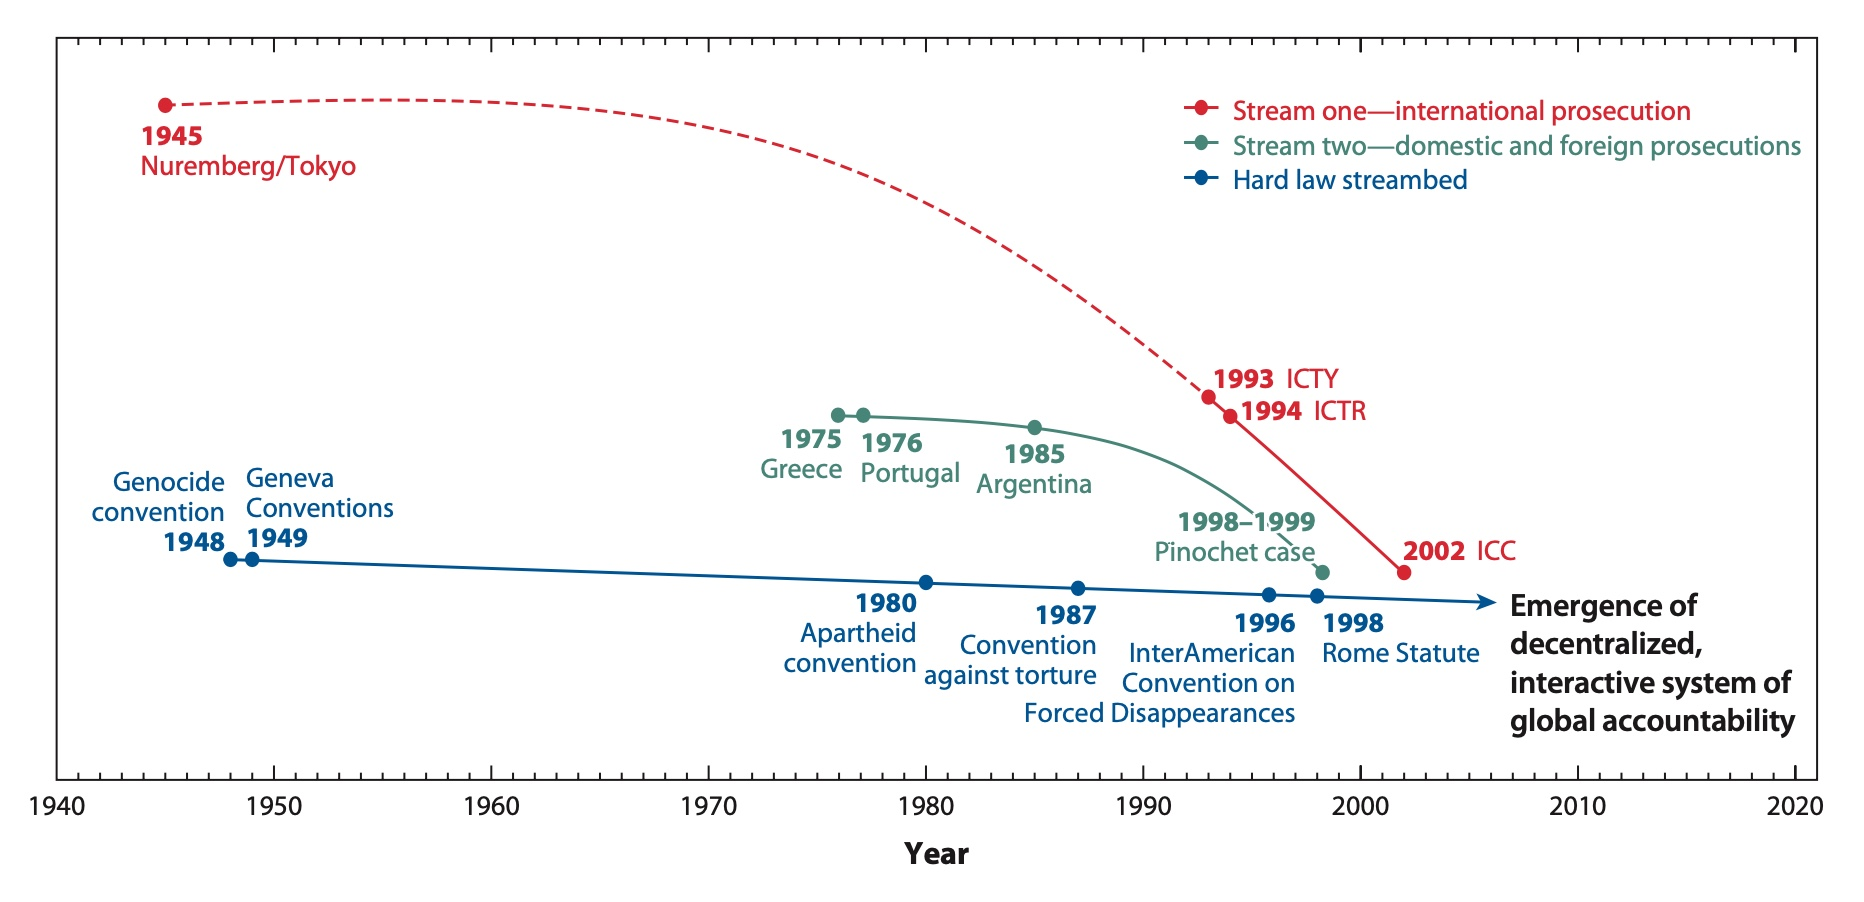
\includegraphics[keepaspectratio, height=0.7\paperheight]{../img/justice_cascade.jpg}};
  \end{tikzpicture}
\end{frame}
% ----------------------------------------------------
\note{El gráfico de Sikkink muestra el crecimiento exponencial de los juicios por DDHH desde los años 80. La tendencia es clara: la cascada. Los juicios domésticos son los más numerosos; los tribunales internacionales y los juicios extranjeros (jurisdicción universal) son más recientes pero también crecen. Preguntar a los estudiantes: ¿qué factores pueden explicar la aceleración a partir de los años 90?}

% ----------------------------------------------------
\begin{frame}
\frametitle{CPI/ICC y TEDH/ECHR: dos modelos de rendición de cuentas}
\centering

\begin{columns}[T]
  \begin{column}{0.47\textwidth}
    \centering
    \textbf{\textcolor{accent}{CPI}} \\
    \textit{\scriptsize Corte Penal Internacional (2002)}
    \vspace{6pt}
    \begin{itemize}
      \item Global: 124 Estados partes
      \item Juzga individuos: genocidio, crímenes de guerra
      \item Complementariedad: solo si el Estado no actúa
      \item Débil: EE.UU., Rusia, China fuera; ¿tribunal africano?
    \end{itemize}
  \end{column}
  \begin{column}{0.47\textwidth}
    \centering
    \textbf{\textcolor{accent2}{TEDH}} \\
    \textit{\scriptsize Convenio Europeo de DDHH (1950)}
    \vspace{6pt}
    \begin{itemize}
      \item Regional: 47 Estados del Consejo de Europa
      \item Petición individual al Tribunal Europeo
      \item Tasa de éxito: $>$50\%; 53.000+ solicitudes/año
      \item El régimen más sólido del mundo
    \end{itemize}
  \end{column}
\end{columns}

\vspace{10pt}
\onslide<2->{\small ¿Por qué el TEDH funciona mejor? Los miembros comparten valores\\y hay costes reales por incumplir}

\end{frame}
% ----------------------------------------------------
\note{El contraste CPI/TEDH es la lección clave de esta sección:
\begin{itemize}
  \item \textbf{CPI:} universalismo vs. soberanía. Alcance global pero sin los Estados poderosos (EE.UU., Rusia, China fuera). La complementariedad reduce su efectividad. Las acusaciones concentradas en África debilitan su legitimidad. La investigación sugiere que las imputaciones de la CPI pueden prolongar conflictos porque los líderes acusados no tienen incentivos para negociar su salida. Primera condena: Thomas Lubanga Dyilo (Congo, 2012), 14 años por usar niños soldados
  \item \textbf{TEDH:} el éxito refleja la homogeneidad de valores entre Estados miembros y los costes reales (reputacionales, económicos) por incumplir. El derecho de petición individual (Protocolo 11, 1998) es su característica más innovadora: cualquier persona puede demandar a su propio Estado ante el Tribunal Europeo
  \item La diferencia no es de diseño sino de contexto: el TEDH opera en un espacio geopolítico cohesionado; la CPI opera en un mundo con grandes potencias y intereses divergentes
\end{itemize}}

% ----------------------------------------------------
\begin{frame}
\frametitle{Justicia transicional: mecanismos}
\centering

\begin{itemize}
  \setlength{\itemsep}{6pt}
  \item<1-> \textbf{Juicios penales:} responsabilidad criminal individual
  \item<2-> \textbf{Amnistías:} olvido legal a cambio de paz (a veces condicional)
  \item<3-> \textbf{Reparaciones:} compensación económica o simbólica a las víctimas
  \item<4-> \textbf{Lustración:} exclusión de exfuncionarios del nuevo régimen
  \item<5-> \textbf{Comisiones de Verdad:} establecer un registro público de lo ocurrido
  \item<6-> \textbf{Memoria y símbolos:} renombrar calles, exhumaciones, monumentos
\end{itemize}

\end{frame}
% ----------------------------------------------------
\note{La justicia transicional es el conjunto de mecanismos que las sociedades usan para gestionar el legado de violaciones masivas de DDHH. Se desarrolló como campo a partir de los años 80-90, durante las transiciones democráticas en América Latina y Europa del Este. No son mecanismos mutuamente excluyentes: muchas sociedades los combinan. Argentina usó juicios y reparaciones. Sudáfrica optó por amnistías condicionales y una comisión de verdad. Alemania hizo todo: juicios (Núremberg), desnazificación (lustración), reparaciones a Israel, y un largo proceso de memoria pública.}

% ----------------------------------------------------
\begin{frame}
\frametitle{Juicios vs.\ amnistías: el dilema}
\centering

\begin{columns}[T]
  \begin{column}{0.47\textwidth}
    \centering
    \textbf{\textcolor{accent}{A favor de los juicios}}
    \begin{itemize}
      \item Justicia para las víctimas
      \item Efecto disuasorio: menos violaciones futuras
      \item Legitimidad del nuevo régimen
      \item La CPI \textbf{prohíbe} amnistías para crímenes bajo su jurisdicción
    \end{itemize}
  \end{column}
  \begin{column}{0.47\textwidth}
    \centering
    \textbf{\textcolor{accent2}{A favor de las amnistías}}
    \begin{itemize}
      \item Facilita las transiciones (los autócratas negocian su salida)
      \item Reduce incentivos para prolongar el conflicto
      \item Pragmatismo: la paz antes que la justicia
    \end{itemize}
  \end{column}
\end{columns}

\vspace{10pt}
\onslide<2->{\small Algunas \textbf{comisiones de verdad} intentan combinar ambas lógicas:\\
verdad a cambio de amnistía condicional}

\end{frame}
% ----------------------------------------------------
\note{El dilema central de la justicia transicional. Los argumentos para los juicios son tanto morales (justicia, verdad, reconocimiento de las víctimas) como instrumentales (disuasión, Sikkink 2011). Los argumentos para las amnistías son pragmáticos: los líderes de un régimen que temen ser juzgados tienen incentivos para no entregar el poder. La Ley de Amnistía española de 1977 fue negociada para facilitar la transición a la democracia. El caso de Colombia y las FARC (2016): el Acuerdo de Paz incluyó un sistema especial de justicia (JEP) con sanciones reducidas a cambio de verdad.}

% ----------------------------------------------------
\begin{frame}
\frametitle{Comisiones de verdad: Argentina y Sudáfrica}
\centering

\begin{columns}[T]
  \begin{column}{0.47\textwidth}
    \centering
    \textbf{\textcolor{accent}{Argentina}}\\
    \textbf{CONADEP (1984)}
    \vspace{6pt}
    \begin{itemize}
      \item Comisión presidencial, no judicial
      \item Investigó la ``Guerra Sucia'' (1976--83)
      \item Informe: \textit{Nunca Más} (1984)
      \item Base para los juicios posteriores
    \end{itemize}
  \end{column}
  \begin{column}{0.47\textwidth}
    \centering
    \textbf{\textcolor{accent2}{Sudáfrica}}\\
    \textbf{Comisión de Verdad y Reconciliación (CVR, 1995--2002)}
    \vspace{6pt}
    \begin{itemize}
      \item Presidida por Desmond Tutu
      \item Amnistía \textit{condicional}: revelar la verdad completa
      \item ``Comprensión, no venganza''
      \item Más de 40 países han adoptado este modelo
    \end{itemize}
  \end{column}
\end{columns}

\end{frame}
% ----------------------------------------------------
\note{Dos modelos de comisiones de verdad:
\begin{itemize}
  \item \textbf{Argentina (CONADEP):} creada por Raúl Alfonsín en 1983. El informe \textit{Nunca Más} documentó 9.000 casos de desaparecidos (la cifra real según organizaciones de DDHH: ~30.000). Sin amnistía: las pruebas recopiladas fueron la base para el Juicio a las Juntas (1985)
  \item \textbf{Sudáfrica (CVR):} modelo de amnistía condicional. Los perpetradores podían solicitar amnistía a cambio de revelación completa y pública de sus crímenes. Desmond Tutu, Premio Nobel de la Paz y arzobispo anglicano, presidió la comisión. Frase famosa: ``No hay futuro sin perdón'' (\textit{No Future Without Forgiveness}, 2000)
\end{itemize}
Más de 40 países han creado comisiones de verdad desde los años 80.}

% ====================================================

% % ----------------------------------------------------
% \begin{frame}
% \centering
% \vspace{2em}

% {\large ¿Juicios, amnistías o comisiones de verdad?}

% \vspace{1.5em}
% \small ¿Qué mecanismo crees que es más eficaz para prevenir futuras violaciones de DDHH?\\[0.5em]
% ¿Y el más justo para las víctimas?

% \end{frame}
% % ----------------------------------------------------
% \note{Pregunta de discusión. Ejes del debate: eficacia vs. justicia; pragmatismo vs. principios; el punto de vista de las víctimas vs. el de los transicionistas. Casos posibles a comparar: Argentina (juicios + verdad), Sudáfrica (verdad + amnistía condicional), España (amnistía sin verdad ni juicios), Colombia (JEP: justicia transicional negociada). Conectar con la Cascada de Justicia: ¿está la norma de accountability desplazando definitivamente a la norma de amnistía?}

% ----------------------------------------------------
\begin{frame}[plain]
  \begin{tikzpicture}[remember picture, overlay]
    \node[at = (current page.center), yshift = 0cm] (cover) {%
      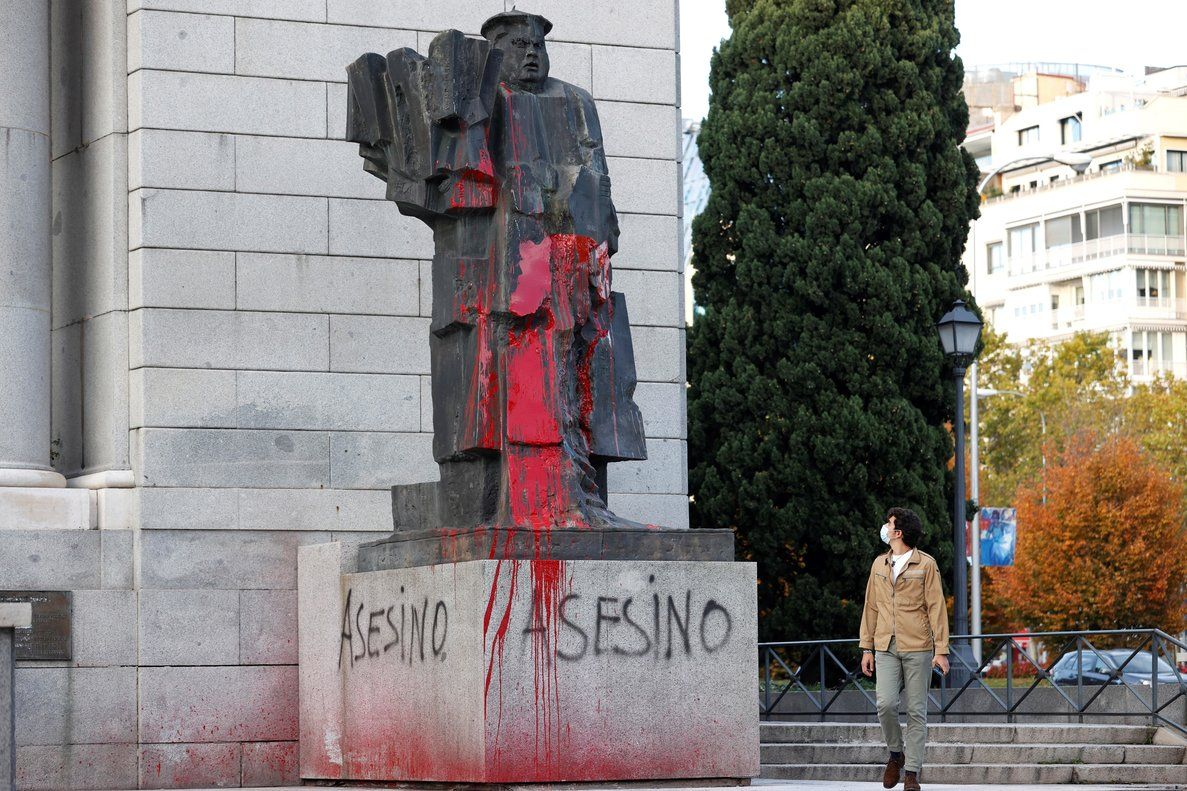
\includegraphics[keepaspectratio, height=\paperheight]{../img/largocaballero}};
  \end{tikzpicture}
\end{frame}
% ----------------------------------------------------
\note{}

% ----------------------------------------------------
\begin{frame}
\frametitle{Resumen: leyes, normas y DDHH en el marco I-I-I}
\centering

\begin{itemize}
  \setlength{\itemsep}{10pt}
  \item \textbf{Intereses:} los Estados crean y cumplen el DI cuando los beneficios de la cooperación superan los costes; los DDHH se violan cuando la supervivencia del régimen está en juego
  \item<2-> \textbf{Interacciones:} la reciprocidad y la reputación hacen cumplir las normas; las TANs activan el efecto bumerán para ejercer presión transnacional
  \item<3-> \textbf{Instituciones:} el DI reduce la incertidumbre y crea expectativas; la CPI y la TEDH institucionalizan la rendición de cuentas; la R2P reconcilia soberanía con DDHH
\end{itemize}

\end{frame}
% ----------------------------------------------------
\note{Cierre del bloque usando el marco I-I-I:
\begin{enumerate}
  \item Intereses: el cumplimiento del derecho internacional es mayor donde los beneficios de la cooperación son claros (comercio, transporte, diplomacia). En DDHH, los intereses son más difusos y los costes de enforcement más altos. Los Estados violan DDHH por supervivencia del régimen, no por indiferencia moral
  \item Interacciones: la reciprocidad (Convenciones de Ginebra, POW) y la reputación (naming \& shaming) son los mecanismos principales. Las TANs reducen los costes de información y activan el efecto bumerán. Las redes sociales han amplificado y acelerado estos efectos
  \item Instituciones: el derecho internacional genera expectativas y define qué es una violación. La CPI pone a individuos (no solo a Estados) ante la rendición de cuentas. La R2P redefine la soberanía como responsabilidad, no como escudo. El TEDH muestra que un sistema robusto es posible cuando hay suficiente homogeneidad de valores y costes reales por incumplir
\end{enumerate}
La próxima sesión: economía política internacional -- pasamos de las reglas de comportamiento a las reglas del comercio y las finanzas.}

% ----------------------------------------------------
\begin{frame}
\frametitle{}
\centering

Preguntas?

\end{frame}
% ----------------------------------------------------
\note{}
